\documentclass[UTF8,a4paper,zihao=-4]{ctexart}

% ==================== 页面与版式 ====================
\usepackage{geometry}
\geometry{a4paper,left=2.5cm,right=2.5cm,top=2.5cm,bottom=2.5cm}
\usepackage{setspace}
\setstretch{1.5}

\usepackage{fancyhdr}
\usepackage{lastpage}


% ==================== 数学 ====================
\usepackage{amsmath}
\usepackage{amssymb}
\usepackage{bm}

% ==================== 图表 ====================
\usepackage{graphicx}
\usepackage{booktabs}
\usepackage{tabularx}
\usepackage{longtable}
\usepackage{multirow}
\usepackage{makecell}
\usepackage{array}
\usepackage{float}
\usepackage{caption}
\usepackage{threeparttable}
\captionsetup{font=small,labelsep=quad}
\captionsetup[table]{position=top,skip=4pt}
\captionsetup[figure]{position=bottom,skip=4pt}
\renewcommand{\arraystretch}{1.25}
\setlength{\tabcolsep}{4pt}
\setlength{\emergencystretch}{2em}

% 图表与公式按节编号，并随节重置
\numberwithin{figure}{section}
\numberwithin{table}{section}
\numberwithin{equation}{section}

% ==================== 列表与标题 ====================
\usepackage{enumitem}
\usepackage{titlesec}
\usepackage{appendix}
\usepackage{chngcntr}


\titleformat{\section}{\centering\bfseries\zihao{4}}{\thesection}{1em}{}
\titleformat{\subsection}{\bfseries\zihao{-4}}{\thesubsection}{1em}{}
\titleformat{\subsubsection}{\bfseries\zihao{-4}}{\thesubsubsection}{1em}{}

\ctexset{
  appendix/name = {附录},
}

% ==================== 算法 ====================
\usepackage{algorithm}
\usepackage{algorithmic}

% ==================== 代码 ====================
\usepackage{xcolor}
\usepackage{listings}
\lstset{
  language=Python,
  basicstyle=\ttfamily\small,
  keywordstyle=\color{blue}\bfseries,
  commentstyle=\color{gray!60},
  stringstyle=\color{gray},
  numbers=left,
  numberstyle=\tiny\color{gray},
  frame=shadowbox,
  rulesepcolor=\color{blue!20},
  breaklines=true,
  tabsize=4,
  showstringspaces=false,
}

% ==================== 参考文献 ====================
\usepackage[super,square]{natbib}
\usepackage[hidelinks,bookmarksnumbered=true]{hyperref}

% ==================== 自定义命令 ====================
\newcommand{\file}[1]{\texttt{#1}}
\newcommand{\R}{\mathbb{R}}
\newcommand{\vx}{\bm{x}}
\newcommand{\vy}{\bm{y}}
\newcommand{\bX}{\bm{X}}
\newcommand{\bY}{\bm{Y}}
\newcommand{\bA}{\bm{A}}
\newcommand{\bR}{\bm{R}}
\newcommand{\bM}{\bm{M}}
\newcommand{\bB}{\bm{B}}
\newcommand{\bD}{\bm{D}}
\newcommand{\bI}{\bm{I}}
\newcommand{\bL}{\bm{L}}
\newcommand{\bP}{\bm{P}}
\newcommand{\bW}{\bm{W}}
\newcommand{\bzero}{\bm{0}}
\newcommand{\bmu}{\bm{\mu}}
\newcommand{\bSigma}{\bm{\Sigma}}
\newcommand{\bbeta}{\bm{\beta}}
\newcommand{\Jcal}{\mathcal{J}}

% ==================== 摘要样式 ====================
\usepackage{abstract}
\renewcommand{\abstractnamefont}{\bfseries\zihao{3}}
\renewcommand{\abstracttextfont}{\zihao{4}\songti}
\setlength{\absleftindent}{0pt}
\setlength{\absrightindent}{0pt}
\setlength{\abstitleskip}{6pt}
% ==================== 论文配图 ====================
\graphicspath{{img/paper/}}
\newcommand{\figinsert}[4][\textwidth]{%
  \begin{figure}[htbp]
    \centering
    \includegraphics[width=#1]{#2}%
    \caption{#3}\label{#4}%
  \end{figure}}

\begin{document}
\thispagestyle{empty}
\begin{center}
\begin{tabular}{|c|c|}
\hline
队伍编号 & MCB2606971 \\
\hline
赛道 & A \\
\hline
\end{tabular}
\end{center}
\vspace{0.8em}
\hrule
\vspace{0.8em}
\begin{center}
{\zihao{-2}\bfseries 啤酒感官评分、关键化合物筛选与风格条件生成}
\end{center}
\vspace{0.2em}
\begin{center}
\textbf{\zihao{3} 摘\quad 要}
\end{center}

针对商用啤酒的化学特征、感官响应与风格生成问题，本文从尺度核验与任务可识别性出发，建立由简单基线到模型比较的流程。
附件实测 \textbf{250 款酒、231 个化学与理化特征、50 个标准化感官响应}；70 个可校准特征中 \textbf{37 列支持 log10、33 列支持线性}，
其余 161 列不作未经验证的浓度反演。外部评论数据仅用于 22 个风格的语义校验，不作逐酒标签补充。

问题一采用\textbf{训练内预处理、选参与选型的嵌套交叉验证}，比较 Ridge、PLS2、ExtraTrees、RandomForest、LightGBM 及融合。
外层 5 折重复 3 次，训练内选型流程的宏平均 $R^2$ 为 \textbf{0.2306}、宏 RMSE 为 \textbf{0.4672}、Spearman 为 \textbf{0.4297}；MCAR 额外 30\% 缺失时 
$R^2$ 相对下降 \textbf{18.42\%}。评分卡 \textbf{52 项中 50 项可监督}、两项乙醛不可识别；以训练分位数锚点给出相对 0--6 等级，\textbf{QWK 为 0.3391}。
该等级非人工绝对分数。

问题二由指定相关表建立 \textbf{Top-10 并集加权图}，得 231 节点、1\,683 边、8 社区，模块度 \textbf{0.5862}；比较边际相关、弹性网、树模型、
SHAP 与图平滑，以平均秩形成候选。主表限定 \textbf{214 个化学候选}，50 个感官目标各取 3 项，500 次全流程 bootstrap 的
平均入选频率为 \textbf{0.4332}、仅 \textbf{19/150 项}达到 0.8；全指标方法间平均 Jaccard 为 \textbf{0.2870}。机理先验仅作敏感性，高重复性不等于因果或最优。

问题三在 70 维校准子谱上比较经验重采样、噪声、\textbf{条件 copula}、协方差匹配与\textbf{正确高斯最优传输}。5 次风格分层留出后，
Tripel、Kriek、Lambic 三风格等权平均的 copula $\mathrm{MMD}^2$ 为 \textbf{0.0445}、覆盖度 \textbf{0.7444}、相对实测画像 RMSE 为 \textbf{0.2919}，
其他模型无全面优势。跨风格迁移以\textbf{超阈值程度不增加}为主约束，11 款 Pils/Lager 到 Tripel 的四类直接化合物均无违反；
反式-2-壬烯醛按两种单位分别计算，stale hops 代理留出能力弱，不宣称整体感官缺陷已受控。

本文给出可追溯的分级、候选与生成结果，同时保留量表、单位与因果辨识的证据边界。

\vspace{0.3em}
\noindent\textbf{关键词：啤酒风味；嵌套验证；共表达网络；bootstrap稳定性；条件copula；高斯最优传输}
\newpage
\pagestyle{empty}
\tableofcontents  


\newpage
\pagestyle{fancy}
\fancyhead{} % 清空页眉所有文字
\renewcommand{\headrulewidth}{0pt} % 去掉页眉那条横线
\pagenumbering{arabic}
\setcounter{page}{1}

% ==================== 1 问题重述 ====================
\section{问题重述}
\label{sec:problem}

\subsection{问题背景}

啤酒的风味、香气与口感由其化学组成决定\cite{liu2023}。酵母在糖代谢中生成乙醇与二氧化碳，并通过酯化反应和氨基酸的 
Ehrlich 降解生成酯类与高级醇；酒花添加带来萜烯、萜醇与异$\alpha$酸；麦芽提供美拉德产物与醛类；
非酿酒酵母与细菌则可能产生双乙酰、4-乙烯基愈创木酚、二甲基硫（DMS）等缺陷物质\cite{guguoxian}。
上述挥发性成分的定量通常依赖固相微萃取与气相色谱--质谱联用\cite{lijj2025}。
同一种化合物在不同浓度区间对感官的贡献方向可能相反，多种化合物之间又存在共同代谢与共表达关系，因此“化合物谱—感官画像”
是一个多变量、非线性的映射问题，仅靠单变量相关分析难以刻画其整体结构。


\subsection{数据说明}
附件给出了 250 个商用啤酒样品\cite{schreurs2024}的化合物丰度、化合物相关矩阵、感官评分卡与感官描述数据。
这批数据覆盖化学测量、感官评价与文本描述三个层面，但并非为同一建模任务整理：化合物列的量纲与变换方式不统一，
感官表只提供标准化后的连续值，跨表主键还存在格式问题。上述特征决定了本文必须先统一数据口径，再针对三问分别建模。

8 份附件数据的内容、规模与本文用途见表~\ref{tab:data}。

\begin{table}[H]
  \centering
  \caption{附件数据一览与本文用途}
  \label{tab:data}
  \small
  \begin{tabularx}{\textwidth}{@{}l >{\hsize=1.2\hsize}X c >{\hsize=0.8\hsize}X@{}}
    \toprule
    文件 & 主要内容 & 规模 & 本文用途 \\
    \midrule
    \file{1.csv} & 250 个啤酒样品的化合物丰度矩阵 & $250\!\times\!234$ & 问题一至三的主特征 \\
    \file{2.csv} & 化合物之间的相关系数矩阵 & $231\!\times\!231$ & 问题二的关联网络 \\
    \file{3.xlsx} & Aroma 与 Flavour 两套评分卡 & 13 个 sheet & 问题一的评分项目与分档定义 \\
    \file{4.csv} & 感官评分的标准化连续值 & $250\!\times\!53$ & 问题一、二的响应取值 \\
    \file{5.csv} & 感官属性之间的相关矩阵 & $50\!\times\!50$ & 感官维度相关结构的核对 \\
    \file{6.csv} & 化合物与感官属性的交叉相关矩阵 & $44\!\times\!50$ & 问题二的同源一致性检查 \\
    \file{7.csv} & 感官描述符与风格标签 & $250\!\times\!189$ & 问题三的风格标签 \\
    \file{8.xlsx} & 感官阈值、校准化学数据与价格等 & 7 个 sheet & 尺度核验与阈值参照 \\
    \bottomrule
  \end{tabularx}
  \par\vspace{3pt}
  \begin{minipage}{\textwidth}
    \footnotesize 注：题面把 \file{3.xlsx} 与 \file{4.csv} 并列为同一批感官品评数据。\file{3.xlsx} 只给出评分项目
    与 0--6 分档，12 张卡都是空白卡，没有已填的分数；与这些项目逐项对应的分数只在 \file{4.csv} 中给出。
    因此本文以 \file{3.xlsx} 定项目与分档、以 \file{4.csv} 定响应取值，没有使用题面之外的数据。
  \end{minipage}
\end{table}

\pagebreak[3]
题面描述与附件实测存在若干出入，本文以附件实测为准：\par\nobreak

\begin{enumerate}[label=（\arabic*）,leftmargin=2.5em,itemsep=0pt,topsep=2pt,parsep=0pt]
  \item 题面称 226 种啤酒，\file{1.csv} 实为 250 个样品；
  \item 题面称 \file{3.xlsx} 含 10 个评分卡，实为 beer\_1 至 beer\_12 共 12 个 sheet 加 1 个 summary；
  \item 题面称两套感官维度共约 40 个。逐项核对评分卡后共整理出 52 个有名称的评分项目：Aroma 与 Flavour 两套合计 30 项，另 20 项可映射到感官结果表，两侧乙醛感官项目 2 项；\file{4.csv} 只对其中 50 项提供标准化连续监督；
  \item 题面称 \file{6.csv} 为 $46\!\times\!50$，实测 44 个指标与 50 个感官属性；
  \item 题面称 \file{7.csv} 为 $250\!\times\!187$，实测 189 列。
\end{enumerate}

后三条直接影响建模：可用的感官维度数、参与交叉相关的指标数、以及风格标签所在的列，都与题面口径不同。其中第（3）条还决定了问题一的交付口径——乙醛在化学特征表中有测量列，却没有对应的两侧感官监督标签，本文不据化学列补造感官标签，两项乙醛保留为“现有数据不可识别”，不计入监督精度。此外，\file{4.csv} 与 \file{7.csv} 的 \file{beer\_id} 有 213/250 行存为科学计数法、仅 96 个唯一值，不能作连接键；本文一律用取值 1--250 且唯一的 \file{beer} 列连接，详见第~\ref{sec:preprocess}~章。

\subsection{问题提出}

\begin{enumerate}[label=（\arabic*）,leftmargin=2.5em,itemsep=2pt]
  \item \textbf{问题一：缺失条件下的感官响应预测与相对分级。}以 \file{1.csv} 的化合物数据为基础，对评分卡中 50 个有监督项目给出连续预测与相对 0--6 等级，两项乙醛保留为不可识别。困难在于标准化响应不唯一决定原始量表、化合物维度 231 与样本数 250 同量级且存在 73 个缺失单元。
  \item \textbf{问题二：化合物关联网络与关键候选筛选。}以 \file{2.csv} 构建化合物关联网络，结合 \file{1.csv} 的特征给出每个感官维度的前三关键候选，并论证其稳定性与化学合理性。困难在于化合物强共线导致候选互相替代，且相关关系不等于因果关系。
  \item \textbf{问题三：风格条件生成与缺陷约束迁移。}以 \file{tasting\_category\_fine} 为风格标签学习条件生成模型，在给定风格（如 Tripel、Kriek、Lambic）下生成化合物谱与感官画像，并完成 Pils/Lager 到 Tripel 的跨风格迁移，保证缺陷化合物不恶化。困难在于 22 个风格样本量悬殊（最多 31 个、最少 3 个），且缺少配对迁移实验与确定的单位口径。
\end{enumerate}

\subsection{技术路线}



\begin{table}[H]
  \centering
  \caption{三问的技术路线}
  \label{tab:roadmap}
  \footnotesize
  \begin{tabularx}{\textwidth}{@{}l >{\hsize=0.82\hsize}X >{\hsize=1.12\hsize}X >{\hsize=1.06\hsize}X@{}}
    \toprule
    问题 & 基线 & 改进 & 最终方案 \\
    \midrule
    问题一 & 总体均值与风格均值 & 多输出正则化与树模型比较 & 训练内选型的等权融合与相对等级 \\
    问题二 & 边际关联排序 & Top-10 并集加权图与一跳平滑 & 五类排序的秩融合与全流程重采样 \\
    问题三 & 经验行重采样与噪声注入 & 条件高斯 copula 与收缩相关 & 高斯最优传输与超阈值程度约束 \\
    \bottomrule
  \end{tabularx}
\end{table}

三问共享同一份原始数据与 \file{beer} 对齐结果，
但本文按不同任务进行对应的预处理：问题一的插补与分位数变换在每个内层、
外层训练集内重新估计；问题二在每次重采样中重新插补、缩放与选参；
问题三在每个风格留出的训练部分拟合尺度、协方差与分位数上限。
这一点与“统一预处理后再建模”的做法不同，
目的是让每一问的结论只依赖它自己的训练信息。
三问的技术路线见表~\ref{tab:roadmap}。输入、建模与产物关系见图~\ref{fig:roadmap}。

\begin{figure}[H]
  \centering
  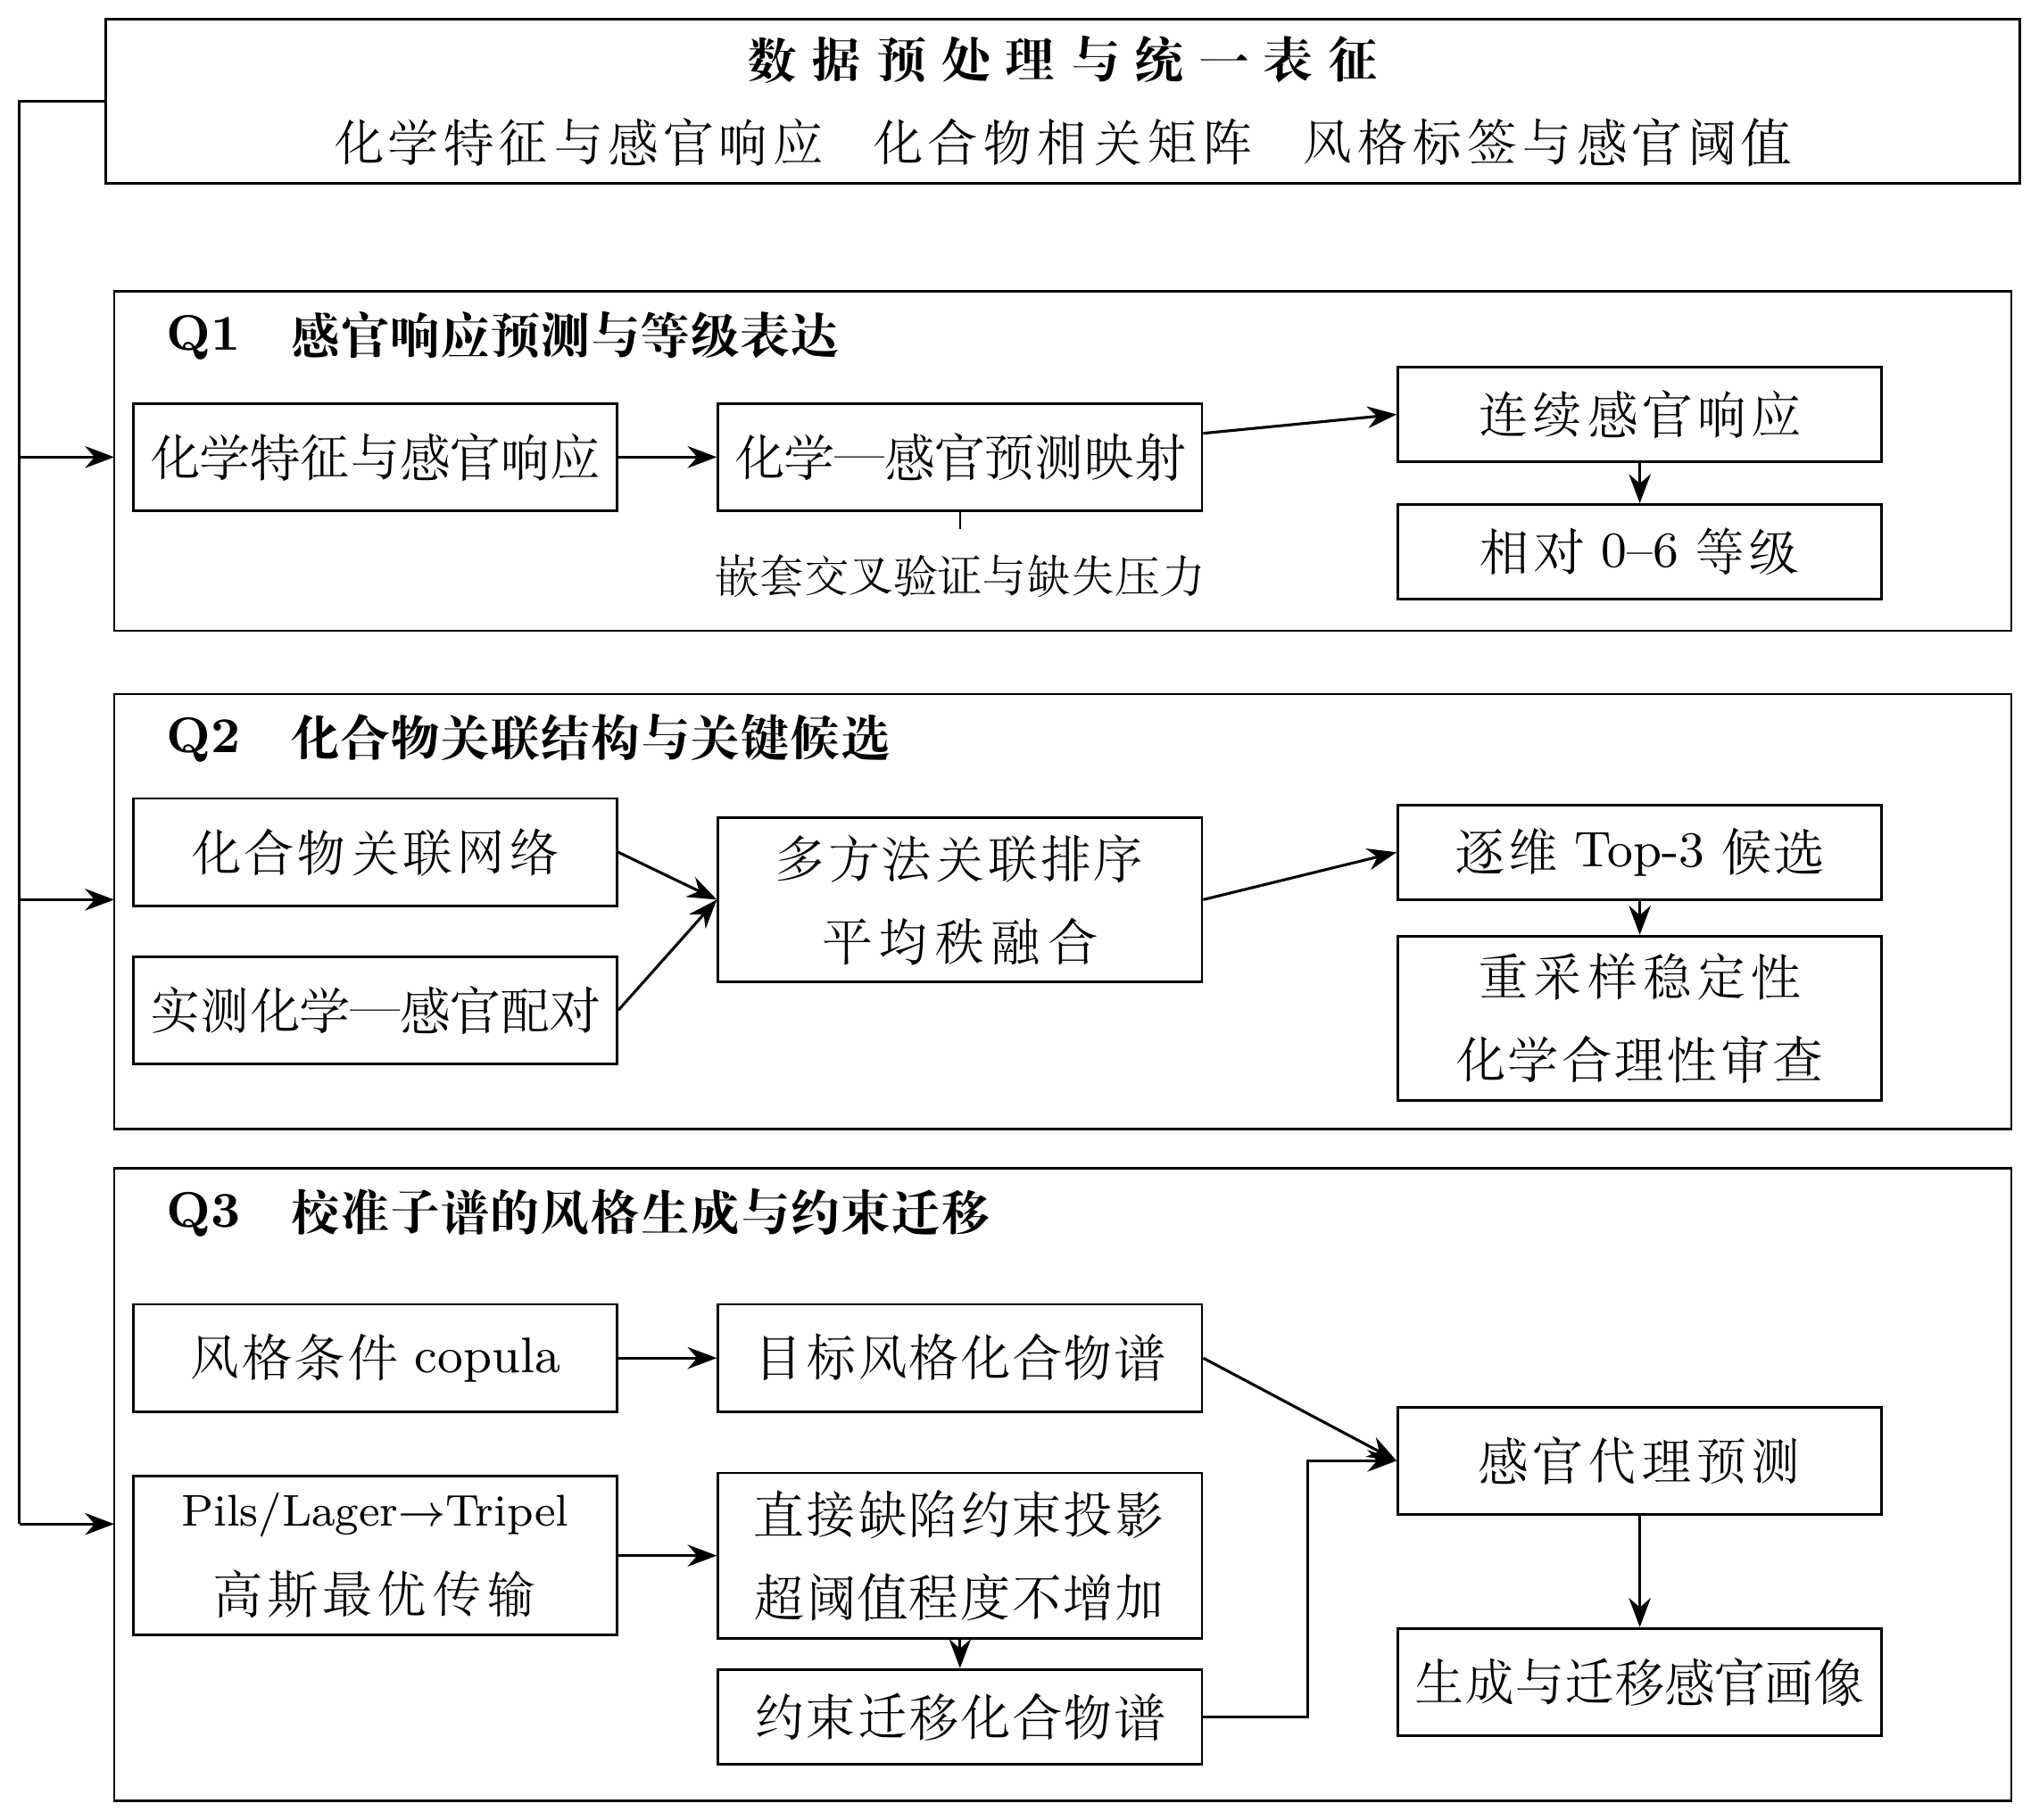
\includegraphics[width=0.9\textwidth]{fig01_roadmap.png}
  \caption{技术路线：以 8 份附件数据为底座，三问分别给出连续预测与相对等级、关联网络与关键候选、条件生成与缺陷约束迁移，并在各自训练划分内完成对照与验证。}
  \label{fig:roadmap}
\end{figure}


% ==================== 2 数据预处理 ====================
\section{数据预处理}
\label{sec:preprocess}

\subsection{模型假设}

以下七条是本文结论成立的前提。它们不是由附件证明的事实，其中多数无法在现有数据上检验，因此每条同时给出依据与失效后果；三问的结论只在这些前提成立时有效。

\begin{enumerate}[label=\textbf{\arabic*},leftmargin=3em,itemsep=2pt,topsep=2pt,parsep=0pt]
 
  \item \textbf{尺度与底数。}各列按第~\ref{sec:scale}~节的核验结果使用：37 列按 log10、33 列按线性，其余 161 列底数未确认，一律不作浓度反演。若这些列的真实底数不同，涉及它们的浓度解释不成立；但基于分位数变换的排序结论不受影响。

  \item \textbf{缺失机制。}MCAR 与按酒精度分层的 MAR 只作为压力测试情景，不代表自然缺失的真实机制。低于检出限的缺失可能与未观测的低浓度有关，而本文缺少检测限元数据，因此不声称对该类缺失无偏。

  \item \textbf{标准化响应与量表。}\file{4.csv} 的标准化响应与原始 0--6 评分只在共同仿射变换下单调对应；若评分先按不同品评员各自缩放再聚合，原始均分的排序未必保留。因此本文只报告相对等级，不称已恢复人工绝对评分。

  \item \textbf{共线结构与关联性质。}感官响应由少量共享化合物因子驱动，但阈值型缺陷维度（\file{barnyard}、\file{clove}、\file{stale\_hops}）不受该共享结构约束；化合物之间的强相关可能来自共同原料、酵母菌株、工艺条件、风格混杂或检测因素，本文不区分其来源，也不据此判断因果方向。

  \item \textbf{生成结构。}同一风格的化合物谱可由“风格原型加风格内相关结构加逐维独立噪声”近似，风格差异主要体现在原型位置。这是小样本下的正则化假设，不是对真实酿造分布的确认；协方差收缩强度是预设值，不由数据证明最优。

  \item \textbf{缺陷代理。}缺陷化合物的浓度与其感官强度在观测范围内单调不减，故“超阈值程度不增加”可作为“缺陷不恶化”的可计算代理。该代理只保证所声明化合物列的变化方向，不保证 \file{stale\_hops}、混合感知或整体风味不恶化。
  
  \item \textbf{样本与风格范围。}250 款样品与 22 个风格可代表附件所覆盖的同类商业啤酒，结论不外推到附件之外的工艺、产区或新风格。\file{Faro} 只有 3 个样本，该风格上的任何结论都只是样本内描述；其余样本量最小的风格同理。

\end{enumerate}

\subsection{符号说明}

本文定义了如下使用次数较多的符号，其余符号在使用时注明。
\begin{table}[H]
  \centering
  \caption{主要符号约定}
  \label{tab:notation}
  \small
  \begin{tabularx}{\textwidth}{@{}l X l@{}}
    \toprule
    符号 & 含义 & 维度/取值 \\
    \midrule
    $N,P,S,G$ & 样本数、化合物数、感官维度数、风格类别数 & — \\
    $i,j,s,g$ & 样本、化合物、感官维度、风格索引 & $i=1,\dots,N$ \\
    $\vx_i$，$\bX$ & 第 $i$ 个样本的特征向量、特征矩阵 & $\R^{P}$，$\R^{N\times P}$ \\
    $y_{i,s}$，$\bY$ & 第 $i$ 个样本第 $s$ 维的响应、响应矩阵 & $\R$，$\R^{N\times S}$ \\
    $\bM$ & 缺失掩码（观测指示） & $\{0,1\}^{N\times P}$ \\
    $z_i$ & 第 $i$ 个样本的风格标签 & $\{1,\dots,G\}$ \\
    $r_{j,j'}$，$\bR$ & 化合物 $j$ 与 $j'$ 的相关系数、相关矩阵 & $[-1,1]$，$\R^{P\times P}$ \\
    $\bA$ & 关联网络的加权邻接矩阵 & $\R^{P\times P}$ \\
    $\bbeta_s$，$\bB$ & 第 $s$ 维的回归系数、系数矩阵 & $\R^{P}$，$\R^{P\times S}$ \\
    $\hat y_{i,s}$ & 第 $i$ 个样本第 $s$ 维的模型预测 & $\R$ \\
    \bottomrule
  \end{tabularx}
\end{table}

\subsection{数据概况与表间对齐}

附件各表的样本标识并不一致。\file{1.csv}、\file{4.csv} 与 \file{7.csv} 都含 \file{beer} 列，取值为 1--250 的唯一编号；而 \file{beer\_id} 在 \file{4.csv} 与 \file{7.csv} 中有 213/250 行被存成科学计数法，仅余 96 个唯一值，无法作为主键。本文因此以 \file{beer} 为唯一连接键建立样本主表，再逐表左连接，连接后核对各列的非空数量与取值范围。原始附件全程只读，不在其中生成任何派生文件。

主表为 250 行、231 个化学与理化特征。自然缺失共 73 个单元（约 0.13\%），集中在 \file{amyl\_acetate}（27）、\file{aroma\_hops\_sum}（13）、\file{methylpyrazine}（12）、\file{2,3-butanedione}（9）与 \file{3-methylbutanal}（7），并非均匀散布。\file{1.csv} 的 231 个特征列与 \file{2.csv} 的行列顺序逐位对应，这一对应关系既是两表可用的前提，也作为读取时的一致性断言。

感官目标共 50 维。各维标准化后的标准差在 0.37--0.86 之间，目标两两相关的中位数仅 0.016，但存在少量强相关对（最高 $r=0.98$）。\file{5.csv} 单独给出的 50 维相关矩阵与之一致：1225 对属性中 $|r|$ 平均 0.170，$|r|\ge0.8$ 的仅 6 对，最强一对为 Stale hops 与 Barnyard（0.966），强相关主要出现在同一物质的香项与味项之间。这说明 50 个维度既不能当作完全独立的任务，也不宜整体视为一个低秩问题。

风格标签共 22 类，样本量高度不均衡：最多的 \file{Blond} 31 个、\file{Tripel} 28 个，最少的 \file{Faro} 仅 3 个。小样本风格在问题三中改用收缩估计，并单独报告其不确定性。

样本量的完整分布见图~\ref{fig:styles}：最多与最少相差约一个数量级。这既是第~5 章采用收缩原型（式~\eqref{eq:shrinkage}）的原因，也是按风格留出评价时必须限制每轮留出数的原因——样本最少的风格只有 3 款，留出 1 款即占三分之一。

\figinsert[0.95\textwidth]{fig17_styles}{%
22 个风格的样本量（按样本数降序）。蓝、橙、绿分别为 \file{Tripel}（28）、
\file{Kriek}（10）、\file{Lambic}（11），金色为 \file{Pils/Lager}（11）；
柱长为实测样本数，不是生成数量。}{fig:styles}

\subsection{尺度核验与使用边界}
\label{sec:scale}

\file{1.csv} 的化合物列并非统一变换。以 \file{8.xlsx} 的校准表为参照，对每个公共特征分别比较线性、$10^{x}$ 与 $e^{x}$ 三种候选在正校准值上的中位相对误差：70 个公共列中 37 列支持 log10 关系、33 列支持线性关系；另外 161 列没有校准依据，本文将其标为底数未确认，不因存在负值或值域较小就执行浓度反演。核验结果与使用边界见表~\ref{tab:transform}。

\begin{table}[H]
  \centering
  \caption{逐列尺度核验及使用边界}
  \label{tab:transform}
  \small
  \begin{tabularx}{\textwidth}{@{}l c >{\hsize=1.15\hsize\raggedright\arraybackslash}X >{\hsize=0.85\hsize\raggedright\arraybackslash}X@{}}
    \toprule
    类别 & 列数 & 判定依据 & 使用方式 \\
    \midrule
    正值区间支持 log10 & 37 & 与校准值的 $10^{x}$ 关系中位相对误差最小 & \file{DMS}、\file{ethyl acetate}、\file{X4VG}、\file{pH} \\
    支持线性 & 33 & 与校准值线性关系中位相对误差最小 & \file{diacetyl}、\file{linalool}、\file{geraniol} \\
    底数未确认 & 161 & 无校准依据 & 不作浓度反演，保留附件原数值 \\
    \bottomrule
  \end{tabularx}
\end{table}

核验中还发现两处不能忽略的细节，它们决定了“反变换”只能作为近似。其一，\file{X4VG} 在校准表中有 168 个零，而对应原表数值的反变换约为 0.00970，并不等于零——说明零值与低值处理还包含未给出的规则，不能把 $10^{x}$ 当作精确可逆映射。其二，\file{pH} 列的原数值与校准 pH 满足 log10 关系，与题面“pH 保留原量纲”的概述存在差异；本文按实测核验结果处理，并在此注明这一冲突。

因此本文不尝试从主特征表统一反演浓度：凡是需要浓度口径的地方（如问题三的缺陷阈值比较），直接使用 \file{8.xlsx} 校准表的对应列，避免把混合尺度的主特征表当成可逆数据源。

关于单位问题，反式-2-壬烯醛在附件中标为 mg/L，但同一列也存在按 $\mu$g/L 理解的可能，两种解读相差 $10^{3}$ 倍，附件中没有可据以判定的校准记录。由于 $0.10\ \mu\mathrm{g/L}=0.00010\ \mathrm{mg/L}$，不能因为数值看起来更合理就选单位：本文以保留附件标注、上限取 0.00010 为主情景，另报告按 $\mu$g/L 解释、上限取 0.10 的替代情景，两种情景的约束与超阈值评价分别计算。

\subsection{缺失值与异常值处理}

预处理按任务分别拟合。问题一在每个内层与外层训练集内做中位数插补与分位数正态化，缺失指示仅作为独立消融，且固定为全部 231 列的观测指示。问题二在每次重采样中重新插补、缩放，并在弹性网选参的内部折中重新拟合插补与标准化。问题三在每个风格留出的训练部分拟合浓度尺度、协方差、经验边际与分位数上限，留出样本不参与这些估计。

缺失机制本身无法从附件中验证，其处理框架按 MCAR 与 MAR 的经典分类展开。本文没有缺失原因的元数据，也没有检测限信息；低于检出限的缺失可能与未观测的低浓度有关，这一点无法用随机遮蔽来检验。因此 MCAR 5\%--30\% 与按酒精度分层的 MAR 只作为压力测试情景使用，不声称自然缺失就是其中任何一种机制。

极端值不单独删除。化合物侧的极端值多对应真实的风味差异（如特种麦芽的高色度、野生菌风格的高挥发酚），删除会连同风格信息一起丢掉；其影响由问题一的分位数正态化与问题三的对数型无量纲变换降低，并在结果中保留极端样本。

\subsection{标准化与特征构造}

两个任务的尺度处理不同，本文在这里分别说明。

问题一对 231 个特征做训练集内的分位数正态化，把每列的经验分布映射到标准正态，从而消除量纲与偏态；插补与变换参数都只在当前折的训练部分估计。

问题三直接使用 \file{8.xlsx} 校准后的 70 个指标。为避免不同量纲改变距离几何，先构造无量纲量再标准化：
\begin{equation}
\ell_{i,j}=\log\left(1+\frac{c_{i,j}}{a_{j}}\right),\qquad
z_{i,j}=\frac{\ell_{i,j}-\mu_{j}}{\sigma_{j}},
\label{eq:q3scale}
\end{equation}
其中 $c_{i,j}$ 为清理后的浓度（负值截断为 0），$a_j$ 为训练集该列正值的中位数，$\mu_j$ 与 $\sigma_j$ 为训练集上的均值与标准差；正值全部缺失的列使用预设回退尺度。单位换算时同步换算 $c$ 与 $a$，使变换不因换单位而改变。

需要强调的是，该处理不把 \file{pH} 等理化指标解释成物质浓度，也不假设不同量纲的列可以任意互换；文中的正则化强度与距离度量，其含义都只限于这里声明的特征空间。

本文没有做 PCA 或自编码器降维：231 维相对于 250 个样本确实偏高，但降维后的成分不再对应任何具体化合物，与问题二、问题三需要指名化合物的要求相冲突，而正则化与低维共享结构已经能承担控制方差的作用。

\subsection{外部数据的使用范围}

题目推荐的外部评论数据取自已公开的 Top Beer Information 数据集（Kaggle 平台），来源为 BeerAdvocate，
许可依既有获取记录记为 CC BY 4.0。该数据在本地取得 5{,}558 行、112 个风格的评论词频记录。

该数据不与附件逐酒合并，附件 250 款酒在全部表格中都没有酒名、酒厂或条码，
Kaggle 一侧也没有条码；退而用同风格且 ABV 相近作代理匹配，
无法确认到具体酒款，因此本文只在风格层级使用它：按互斥语义规则把 112 个原风格中的 96 个映射到附件的 22 类，映射覆盖 4{,}760 行（85.6\%）；11 列词频按每行总词频归一化，剔除总词频小于 50 的行后，映射范围内保留 4{,}492 行，按风格聚合为 22 个感官词频原型。映射规则、原型构造与过滤由同一脚本执行，不依赖手工填入的原型表。

该数据只用于风格级外部校验，没有进入问题一的风格编码，也没有用于问题三的生成分布或迁移方向估计。以 \file{7.csv} 的风格均值作对照，风格级酸感、酒花与麦芽词频的相关分别约为 0.890、0.818 与 0.799；这些相关只建立在 22 个风格上，属于生态相关，词频比例也不等于训练面板的强度或 0--6 评分，语义映射更不是官方的风格等价关系，因此不能外推到逐酒预测。

\section{问题一：缺失条件下的感官响应预测与相对分级}
\label{sec:q1}

\subsection{问题分析}

本文以 250 个样本、231 个化学与理化特征预测 50 维标准化感官响应。逐项核对评分卡后共整理出 52 个有名称的评分项目：麦芽、酒花与酯类的 Aroma/Flavour 项目合计 30 项，其他可映射到感官结果表的项目 20 项，以及两侧乙醛感官项目 2 项。\file{4.csv} 只对这 50 项提供标准化连续监督；乙醛在化学特征表中有测量列，却没有对应的两侧感官监督标签，本文不据化学列补造感官标签。两项乙醛因此保留为“现有数据不可识别”，不计入监督精度。

标准化响应不唯一决定原始 0--6 量表。若观测值满足 $y=(k-a)/b$ 且 $b>0$，未知的中心 $a$ 与尺度 $b$ 仍使绝对档位无法由 $y$ 唯一确定；若评分先按不同品评员各自缩放再聚合，原始均分的排序也不必严格保留。本文因此把连续预测与相对等级分开评价，不报告人工档位准确率，也不把 0--6 输出称为已恢复的原始评分。

高维共线需要控制估计方差，但这一事实并不推出必须使用某一种复杂模型。231 个特征对应 250 个样本，同源化合物高度相关，逐维最小二乘的方差很大。本文先建立两类不含化学信息的基线，再比较候选学习器，并把“化学特征是否提供风格之外的增益”作为主要判据。

\subsection{评价指标}

连续指标先按目标计算再取宏平均。均方根误差定义为
\begin{equation}
\mathrm{RMSE}_{\mathrm{macro}}=\frac{1}{S}\sum_{s=1}^{S}\sqrt{\frac{1}{n}\sum_{i=1}^{n}\left(\hat y_{i,s}-y_{i,s}\right)^{2}},
\label{eq:rmse-macro}
\end{equation}
即先对每个目标开方、再跨目标平均，与“先合并全部平方误差再开方”的池化 RMSE 不是同一量。平均绝对误差按样本与维度平均；决定系数先逐维计算再平均：
\begin{equation}
\bar R^{2}=\frac{1}{S}\sum_{s=1}^{S}\left(1-\frac{\sum_{i=1}^{n}(y_{i,s}-\hat y_{i,s})^{2}}{\sum_{i=1}^{n}(y_{i,s}-\bar y_{s})^{2}}\right).
\label{eq:r2-macro}
\end{equation}
排序一致性用 Spearman 秩相关，计算时对并列值取平均秩后按 Pearson 相关系数求值——存在并列时，这与直接套简化公式并不等价。

分级一致性用二次加权 Kappa\cite{cohen1968}。设 $O_{k,k'}$ 为参考等级 $k$ 被判为 $k'$ 的频数，期望频数取行边际与列边际之积除以总数，$W_{k,k'}=(k-k')^{2}/36$，则
\begin{equation}
\mathrm{QWK}=1-\frac{\sum_{k=0}^{6}\sum_{k'=0}^{6}W_{k,k'}O_{k,k'}}{\sum_{k=0}^{6}\sum_{k'=0}^{6}W_{k,k'}E_{k,k'}}.
\label{eq:qwk}
\end{equation}
只要分母非零，恒定预测得到的零分仍纳入统计，不能因该目标无法分档就把它剔除，否则会虚高 QWK。

\subsection{模型构建}

\subsubsection{基线模型：总体均值与风格均值}

第一个基线不使用任何特征，只取训练目标均值 $\bar y_s$。第二个基线只使用 \file{1.csv} 自带的风格标签，对风格 $g$ 取风格均值与总体均值的平滑混合：
\begin{equation}
\hat y_{g,s}=\frac{n_{g}\bar y_{g,s}+\kappa\bar y_{s}}{n_{g}+\kappa},\qquad \kappa=5,
\label{eq:style-baseline}
\end{equation}
其中 $n_g$ 为训练部分中风格 $g$ 的样本数。取 $\kappa=5$ 是因为样本最少的 \file{Faro} 只有 3 个样本，不收缩会让它的预测完全由这 3 款酒决定；训练部分未出现的风格回退到 $\bar y_s$。这个基线比总体均值严格得多：它承认“知道风格即已知大部分感官期望”，化学特征必须在它之上仍然带来增益，才说明化合物谱提供了风格之外的信息。

\subsubsection{候选学习器与融合}

比较 Ridge、PLS2、ExtraTrees、RandomForest 与逐目标 LightGBM。前两者的正则化路径见文献\cite{lihang}，
随机森林与梯度提升的构造见文献\cite{zhouzhihua}，PLS2 的提取准则见文献\cite{wanghuiwen}。Ridge 通过系数平方惩罚控制高维共线；在给定正则化强度后，其目标可按感官维度分解，因此不能称为直接利用目标协方差的联合约束。PLS2 以少量共享成分刻画化学与感官的协变，是否合适由留出误差决定，不由少数强相关对证明。

融合取两种：两模型平均（Ridge 与 ExtraTrees）与五模型平均（全部五类的等权均值）：
\begin{equation}
\hat y_{i,s}^{\mathrm{avg}}=\frac{1}{|\mathcal{M}|}\sum_{\nu\in\mathcal{M}}\hat y_{i,s}^{(\nu)}.
\label{eq:fusion}
\end{equation}
等权不引入额外的权重估计，但不保证优于单体。另以固定正则化强度 1 的逐目标 Ridge 堆叠作对照，其元特征只来自当前外层训练部分的内部折外预测，绝不把全数据主交叉验证的折外行回流进来。

\subsubsection{相对等级与校准敏感性}

主报告规则采用外层训练目标的 1\% 与 99\% 分位数作为锚点：
\begin{equation}
\hat k_{i,s}=\operatorname{clip}_{[0,6]}\left[\operatorname{round}\left(6\cdot\frac{\hat y_{i,s}-q_{01,s}}{q_{99,s}-q_{01,s}}\right)\right].
\label{eq:grade}
\end{equation}
同一外层测试集的参考等级也由同一训练锚点映射其连续观测值，不使用全样本分位数。该规则只规定相对报告尺度，不能把 0 级与 6 级解释为已校准到原始人工极端档位。

另比较保序、线性重标、预测分位数映射、固定分布分位数分档与高斯潜变量五种替代规则。需要学习的映射只在当前外层训练部分的内部折外预测上拟合，外层测试不参与模型、超参数或校准选择；所有规则都对同一训练锚点参考等级评价，不为每种规则另换一个“真值”。保序回归允许平台合并，不能保证严格保留每个名次；连续预测向均值收缩也可能是条件均值的合理性质，不据尾部频数单独判定模型失败。

\subsection{实验设置}

外层为随机种子 42 的 5 折交叉验证、重复 3 次，共 15 折，每折训练 200、测试 50；内层 3 折，插补与分位数变换在各内层训练部分重新拟合。Ridge 正则化强度遍历 $10^{0},10^{1},\dots,10^{6}$；PLS 成分数取 2、4、8、12；ExtraTrees 最小叶样本数取 1、3、6，RandomForest 取 2、4；树模型内部选参用 200 棵、外层重拟合用 500 棵；LightGBM 固定 250 棵、学习率 0.03、叶数 10、最小叶样本 15、行与列采样各 0.8。

每个外层训练集先得到候选学习器与两个平均融合的内层折外预测，按训练内宏平均 $R^2$ 选定该折的学习器，再重新拟合并预测外层测试。本文主结果评价的是这一预先声明的选型流程，而不是查看 15 个测试折之后再宣布某个单体最优——后者会让选型本身成为信息泄漏。15 折中，训练内流程有 14 折选中五模型平均、1 折选中 ExtraTrees。

\subsection{结果与分析}

15 折结果见表~\ref{tab:q1-results}。

\begin{table}[H]
  \centering
  \caption{相同外层 15 折下的连续响应预测（数值为折均值）}
  \label{tab:q1-results}
  \small
  \begin{tabularx}{\textwidth}{@{}>{\raggedright\arraybackslash}X c c c c@{}}
    \toprule
    方法 & $\bar R^{2}$ & MAE & 宏 RMSE & 平均 Spearman \\
    \midrule
    总体均值 & $-0.0289$ & 0.4174 & 0.5620 & — \\
    仅风格均值 & 0.1423 & 0.3638 & 0.5019 & 0.3557 \\
    Ridge & 0.1454 & 0.3641 & 0.4931 & 0.3638 \\
    PLS2 & 0.1442 & 0.3659 & 0.4937 & 0.3748 \\
    ExtraTrees & 0.2201 & 0.3420 & 0.4711 & 0.4281 \\
    RandomForest & 0.2176 & 0.3432 & 0.4729 & 0.4187 \\
    LightGBM & 0.1772 & 0.3481 & 0.4778 & 0.3946 \\
    两模型平均 & 0.2132 & 0.3453 & 0.4736 & 0.4167 \\
    五模型平均 & 0.2314 & 0.3398 & 0.4670 & 0.4310 \\
    训练内折外堆叠 & 0.2256 & 0.3376 & 0.4657 & 0.4226 \\
    训练内选型流程 & 0.2306 & 0.3399 & 0.4672 & 0.4297 \\
    ExtraTrees 加缺失指示 & 0.2214 & 0.3417 & 0.4708 & 0.4295 \\
    Ridge 加风格独热 & 0.1460 & 0.3640 & 0.4929 & 0.3642 \\
    \bottomrule
  \end{tabularx}
\end{table}

训练内选型流程的宏平均 $\bar R^2$ 为 0.2306、宏 RMSE 为 0.4672、平均 Spearman 为 0.4297，$\bar R^2$ 与宏 RMSE 的折间标准差分别为 0.0217 与 0.0181。五模型平均（0.2314）比最强单体 ExtraTrees（0.2201）高 0.0113；两模型平均（0.2132）反而低于 ExtraTrees 的单独表现；训练内堆叠的 $\bar R^2$（0.2256）低于五模型平均，MAE（0.3376）与宏 RMSE（0.4657）却更低。三种融合方式之间没有一致的胜负关系。

化学特征的增益主要体现在与总体均值（$-0.0289$）的差距上；相对仅风格均值（0.1423），选型流程只高出 0.0883。

为了判断 0.0883 是否稳定，我们采用另一种聚合口径：把每款酒三次折外预测先取平均，再在 250 款酒上做配对 bootstrap 2000 次。该口径逐酒聚合，与表~\ref{tab:q1-results} 的“先按折求指标、再跨折平均”不是同一估计量，其主流程宏 $\bar R^2$ 为 0.2587，与表内 0.2306 不可互相代入。同一口径下，主流程相对仅风格均值差 0.0891、95\% 条件区间 $[0.0692,0.1090]$；相对 ExtraTrees 差 0.0110、区间 $[0.0034,0.0184]$；相对五模型平均的差约 0.00006、区间跨零。两个口径的差值与表内 0.0883、0.0105 方向一致、量级相当。该区间条件于已拟合的交叉验证预测，不含重新训练与模型开发的不确定性。

两项消融都没有实质贡献：ExtraTrees 加缺失指示为 0.2214，不加为 0.2201；Ridge 加风格独热为 0.1460，不加为 0.1454。自然缺失下缺失模式携带的信息有限，风格标签在该编码下也基本冗余。

在同一参考等级下，预设分位数规则的 QWK 为 0.3391、等级 MAE 为 0.8252，保序重标为 0.3731 与 0.8286，线性重标为 0.3534 与 0.8208，预测分位数映射为 0.4551 与 0.9346。QWK 更高并未换来更小的档位误差，因此本文以预设规则作为报告尺度，其余只作敏感性分析，不声称已经确定最佳的人工评分校准。

最终相对等级取三次外层报告等级的中位数；250 款、52 项的完整输出见支撑材料，其中 500 个乙醛栏位（250 款 $\times$ 2 项）标注为无可识别分数。

交付格式见图~\ref{fig:card}：52 项按评分卡版面排布，50 项给出相对 0--6 等级，两侧乙醛保留为空。

\begin{figure}[H]
  \centering
  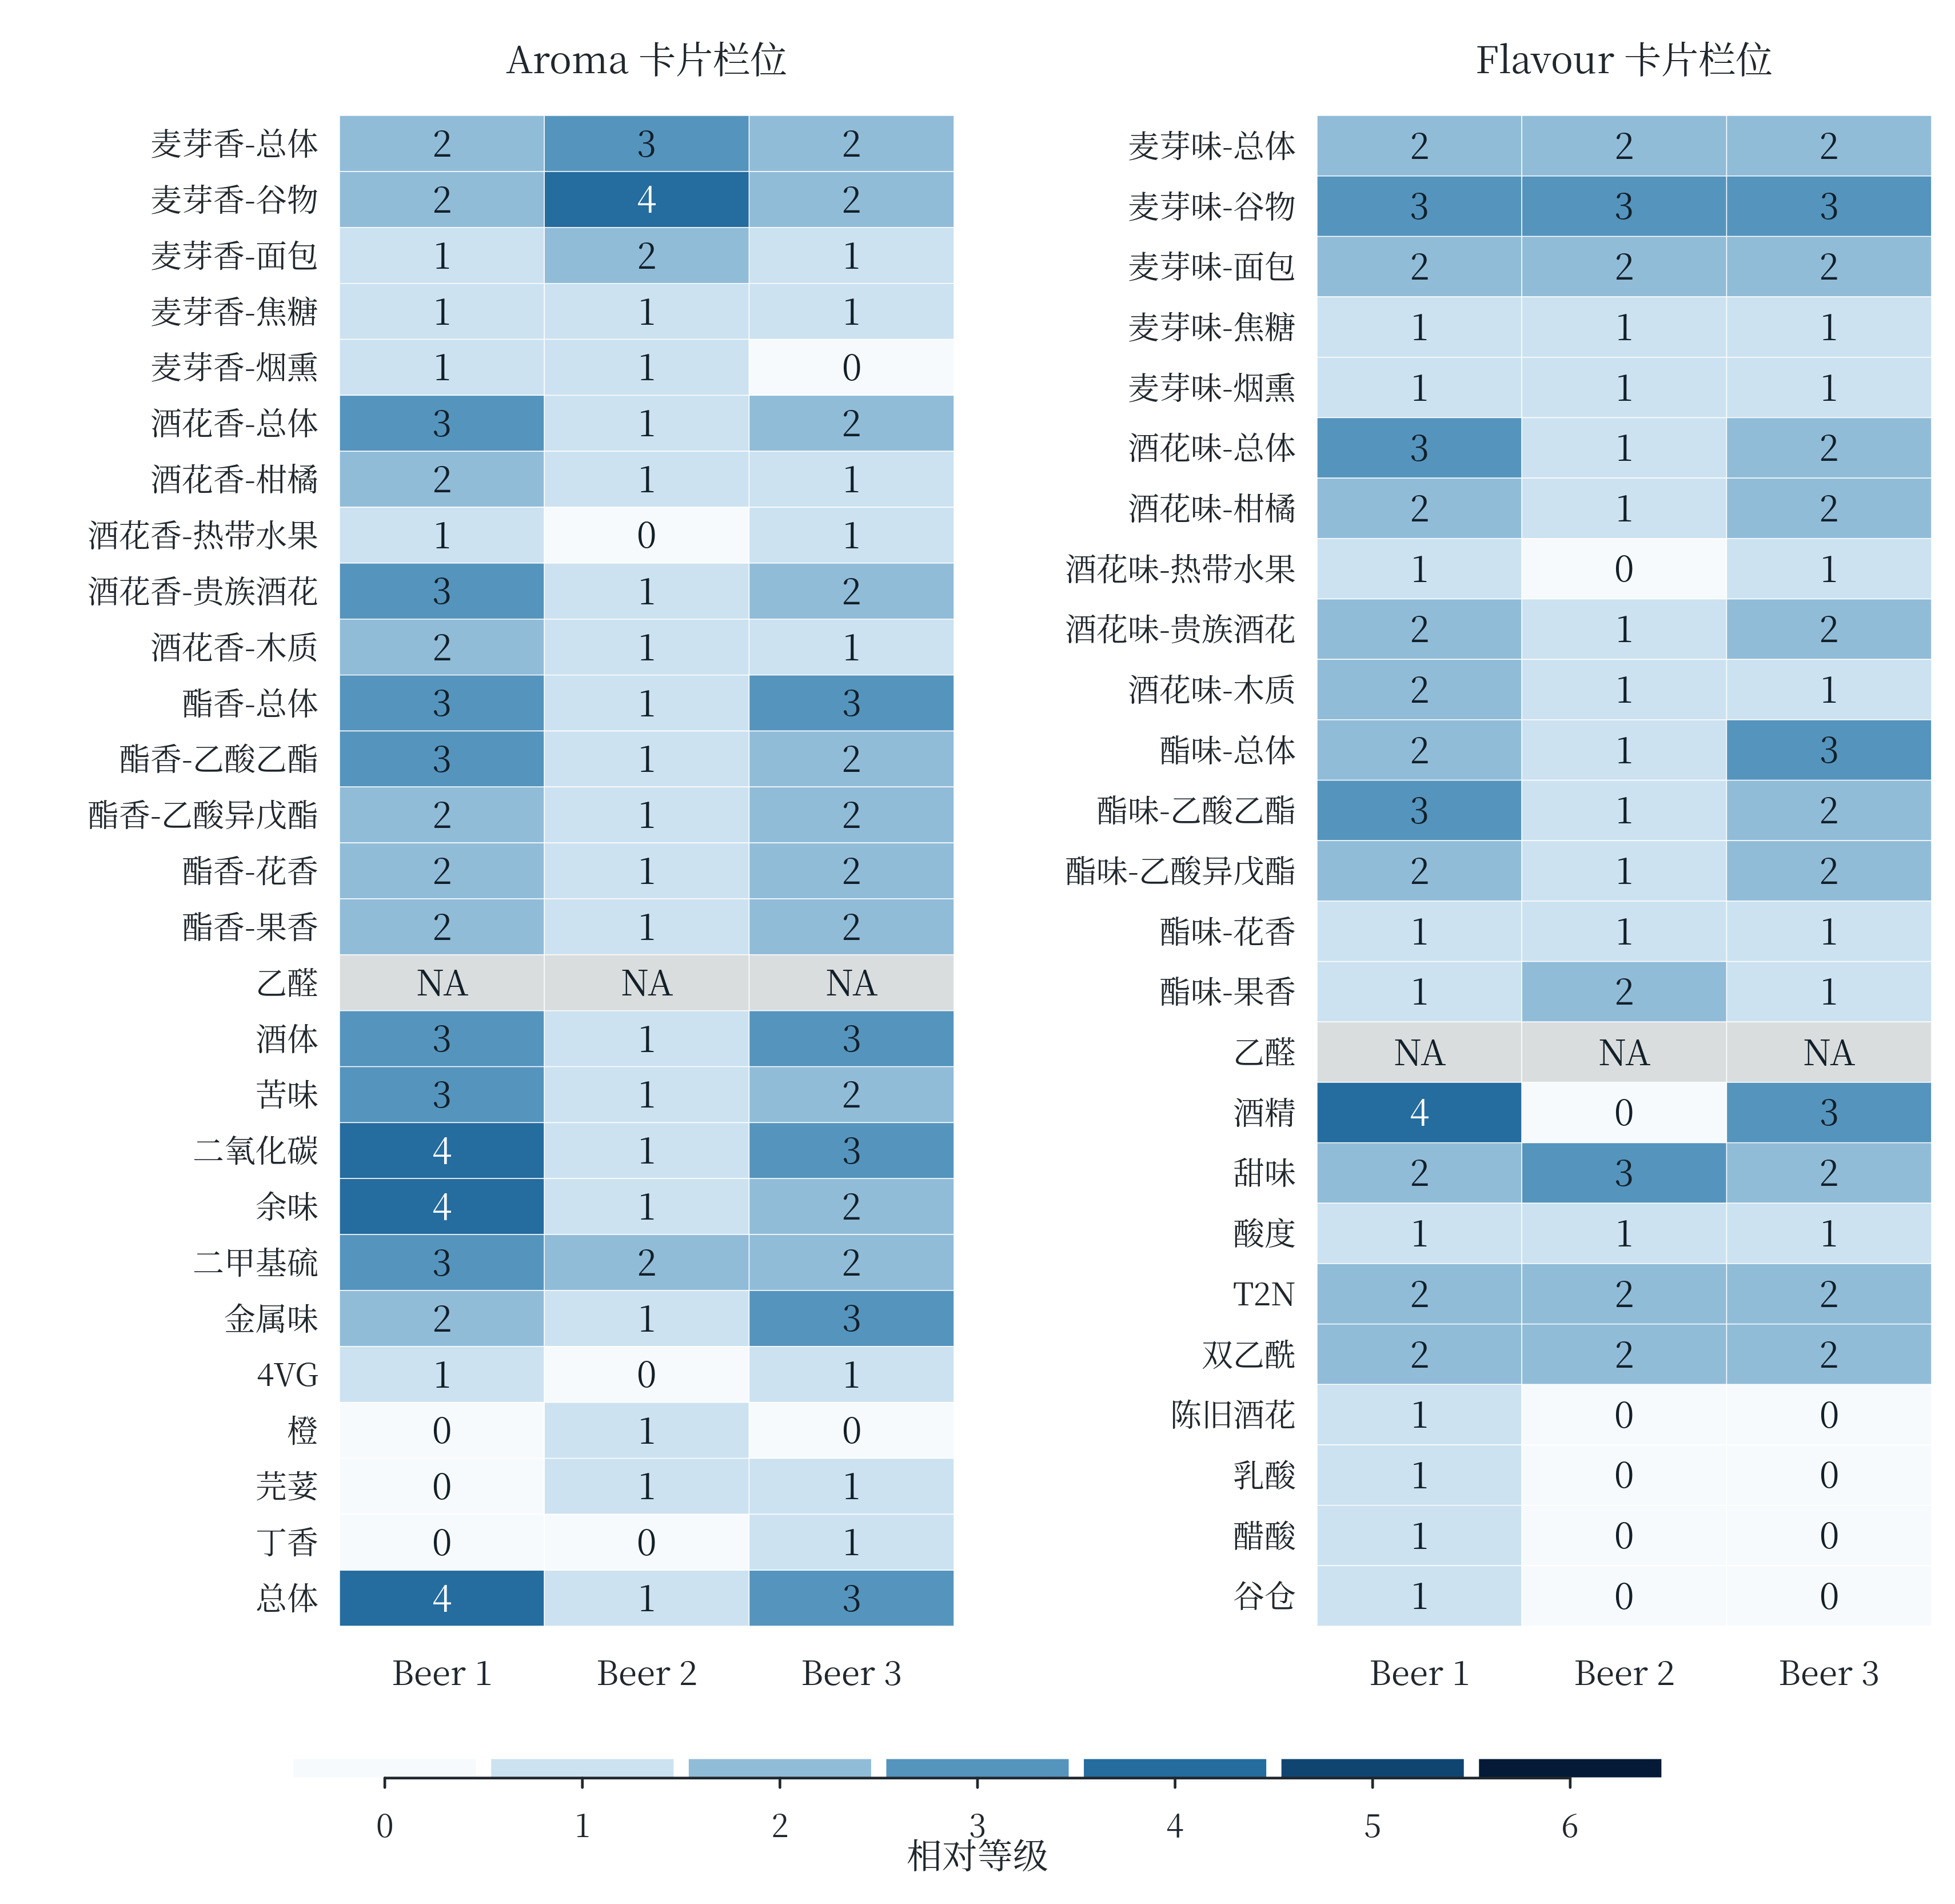
\includegraphics[width=\textwidth]{fig03_card.png}
  \caption{评分卡位置输出示例（Beer 1--3，共 52 项）。30 项 Aroma/Flavour 项目与 20 项可映射项目给出相对 0--6 等级；两侧乙醛 2 项保留为空，标注为现有数据不可识别。等级为训练锚点下的相对尺度，不是人工原始评分。完整 250 款 $\times$ 52 项见支撑材料。}
  \label{fig:card}
\end{figure}


\subsection{缺失压力测试}

每个外层训练模型保持冻结，只遮蔽其测试特征。MCAR 追加 5\%、10\%、20\%、30\% 随机缺失；MAR 按训练酒精度四分位数确定测试样本的缺失概率 0.05、0.15、0.30、0.50，且酒精度驱动列本身不遮蔽。两者都叠加在自然缺失之上，故名义比例与实测总比例略有差异。

自然缺失下主流程 $\bar R^2=0.2306$；MCAR 的实测总缺失约 5.06\%、10.09\%、20.19\%、30.15\%，$\bar R^2$ 相对下降 1.23\%、4.70\%、10.74\%、18.42\%；MAR 的总缺失约 25.04\%，相对下降 11.97\%。

这些结论只适用于所设的遮蔽机制：它不证明自然缺失就是 MAR，也不证明模型对检测限导致的非随机缺失无偏。

\subsection{讨论}

问题一的主要困难是可识别性。标准化响应无法唯一决定绝对档位，换成有序模型或更复杂的校准都不能凭空补回锚点；要报告绝对等级精度，必须取得原始评分、锚定实验或专家复核数据。

其次是“最优”的边界。本文能证明的是：在预先声明的选型流程与候选集合内，含化学特征的模型优于两类无化学基线，五模型平均略优于最强单体。这不足以支撑“五模型等权最优”——两模型平均下降、堆叠在部分指标更好，都说明融合方式的选择依赖评价口径。

最后是缺失机制。随机遮蔽与按酒精度分层的 MAR 只能作为压力测试情景，不能验证真实缺失机制；未检出缺失可能与低浓度有关，而本文缺少检测限元数据。%有一种改法叫没有给出检出限，这个词其实更难理解，建议保留

% ==================== 4 问题二 ====================
\section{问题二：化合物关联网络与关键候选筛选}
\label{sec:q2}

\subsection{问题分析}

本文把“关键因素化合物”操作化为多种关联与预测归因方法共同支持的候选：先用给定相关矩阵建立关联网络刻画模块结构\cite{wangxiaofan}，再用五类方法各自排序并以平均秩融合，最后用重采样\cite{maosongsong}衡量选择稳定性、用化学知识审查合理性。这一定义不等于干预因果效应：高度共线的同族化合物可能互相替代，入选频率低也不等于没有风味作用。

候选范围需要先说清。附件 231 列中有 13 列被元数据归为理化指标、4 列为派生指数，主表把 Top-3 限定在其余 214 个化学候选中，每个感官维度保留 3 项。所有方法先对 231 列计算排名，再在化学候选中截取，因此这是“化学候选下的条件筛选”，不是假装重新拟合了一个 214 维模型。理化与派生指标的全量排名、Top-3 与稳定性另列为诊断表，以免把 pH、蛋白或色度直接称作化合物。

\subsection{评价指标}

本题没有预测精度意义上的真值，评价分三层：排序层用 500 次重采样下候选的入选频率，一致层用方法之间 Top-3 集合的 Jaccard 系数，用途层用训练内选出的前三变量训练固定读出器并评价留出响应。三层回答不同问题，不能互相替代。

入选频率定义为
\begin{equation}
\hat\pi_{j,s}=\frac{1}{500}\sum_{b=1}^{500}\mathbf{1}\left\{j\in\operatorname{Top3}_{\mathrm{chem}}(\mathcal{D}_b)\right\},
\label{eq:freq}
\end{equation}
其中 $\mathcal{D}_b$ 为第 $b$ 次重采样得到的酒样集合。频率只表示当前抽样与选择规则下的重复性，不是“为真的概率”；由于 \file{2.csv} 作为给定先验固定，频率条件于该图，并未覆盖重建图带来的不确定性。方法一致性用两两 Jaccard 系数
\begin{equation}
J\left(\mathcal{T}^{(\nu)},\mathcal{T}^{(\nu')}\right)=\frac{\left|\mathcal{T}^{(\nu)}\cap\mathcal{T}^{(\nu')}\right|}{\left|\mathcal{T}^{(\nu)}\cup\mathcal{T}^{(\nu')}\right|}.
\label{eq:jaccard}
\end{equation}

\subsection{模型构建：从相关图到平均秩融合}

\subsubsection{给定相关图及其局限}

题目把 \file{2.csv} 描述为 Pearson 矩阵，逐项核验却发现它与按并列秩计算的 Spearman 相关矩阵在 $10^{-8}$ 容差内一致；本文仍使用题目指定的 \file{2.csv} 构图，并按实测性质称之为秩相关。

设 $r_{j,k}$ 为给定矩阵元素，$N_{10}(j)$ 为除自身外绝对相关最大的 10 个邻居，采用 Top-10 并集的加权邻接：
\begin{equation}
A_{j,k}=\left|r_{j,k}\right|\cdot\mathbf{1}\left\{k\in N_{10}(j)\ \text{或}\ j\in N_{10}(k)\right\},\qquad A_{j,j}=0.
\label{eq:adj}
\end{equation}
邻接取绝对值，原始正负号另作保留。每个节点至少保留 10 个邻居，不代表这些边都强或都显著。

以加权 Louvain 划分社区\cite{blondel2008}，主图得到 231 个节点、1\,683 条边、8 个社区，模块度 0.5862（图~\ref{fig:q2net}）。Top-5 图的模块度更高，硬阈值 $|r|\ge0.5$ 则产生 48 个孤立点；这说明模块度与连通性都不能单独作为“图构造最优”的依据，社区反映的是相关模块，也可能受风格混杂影响。

\begin{figure}[H]
  \centering
  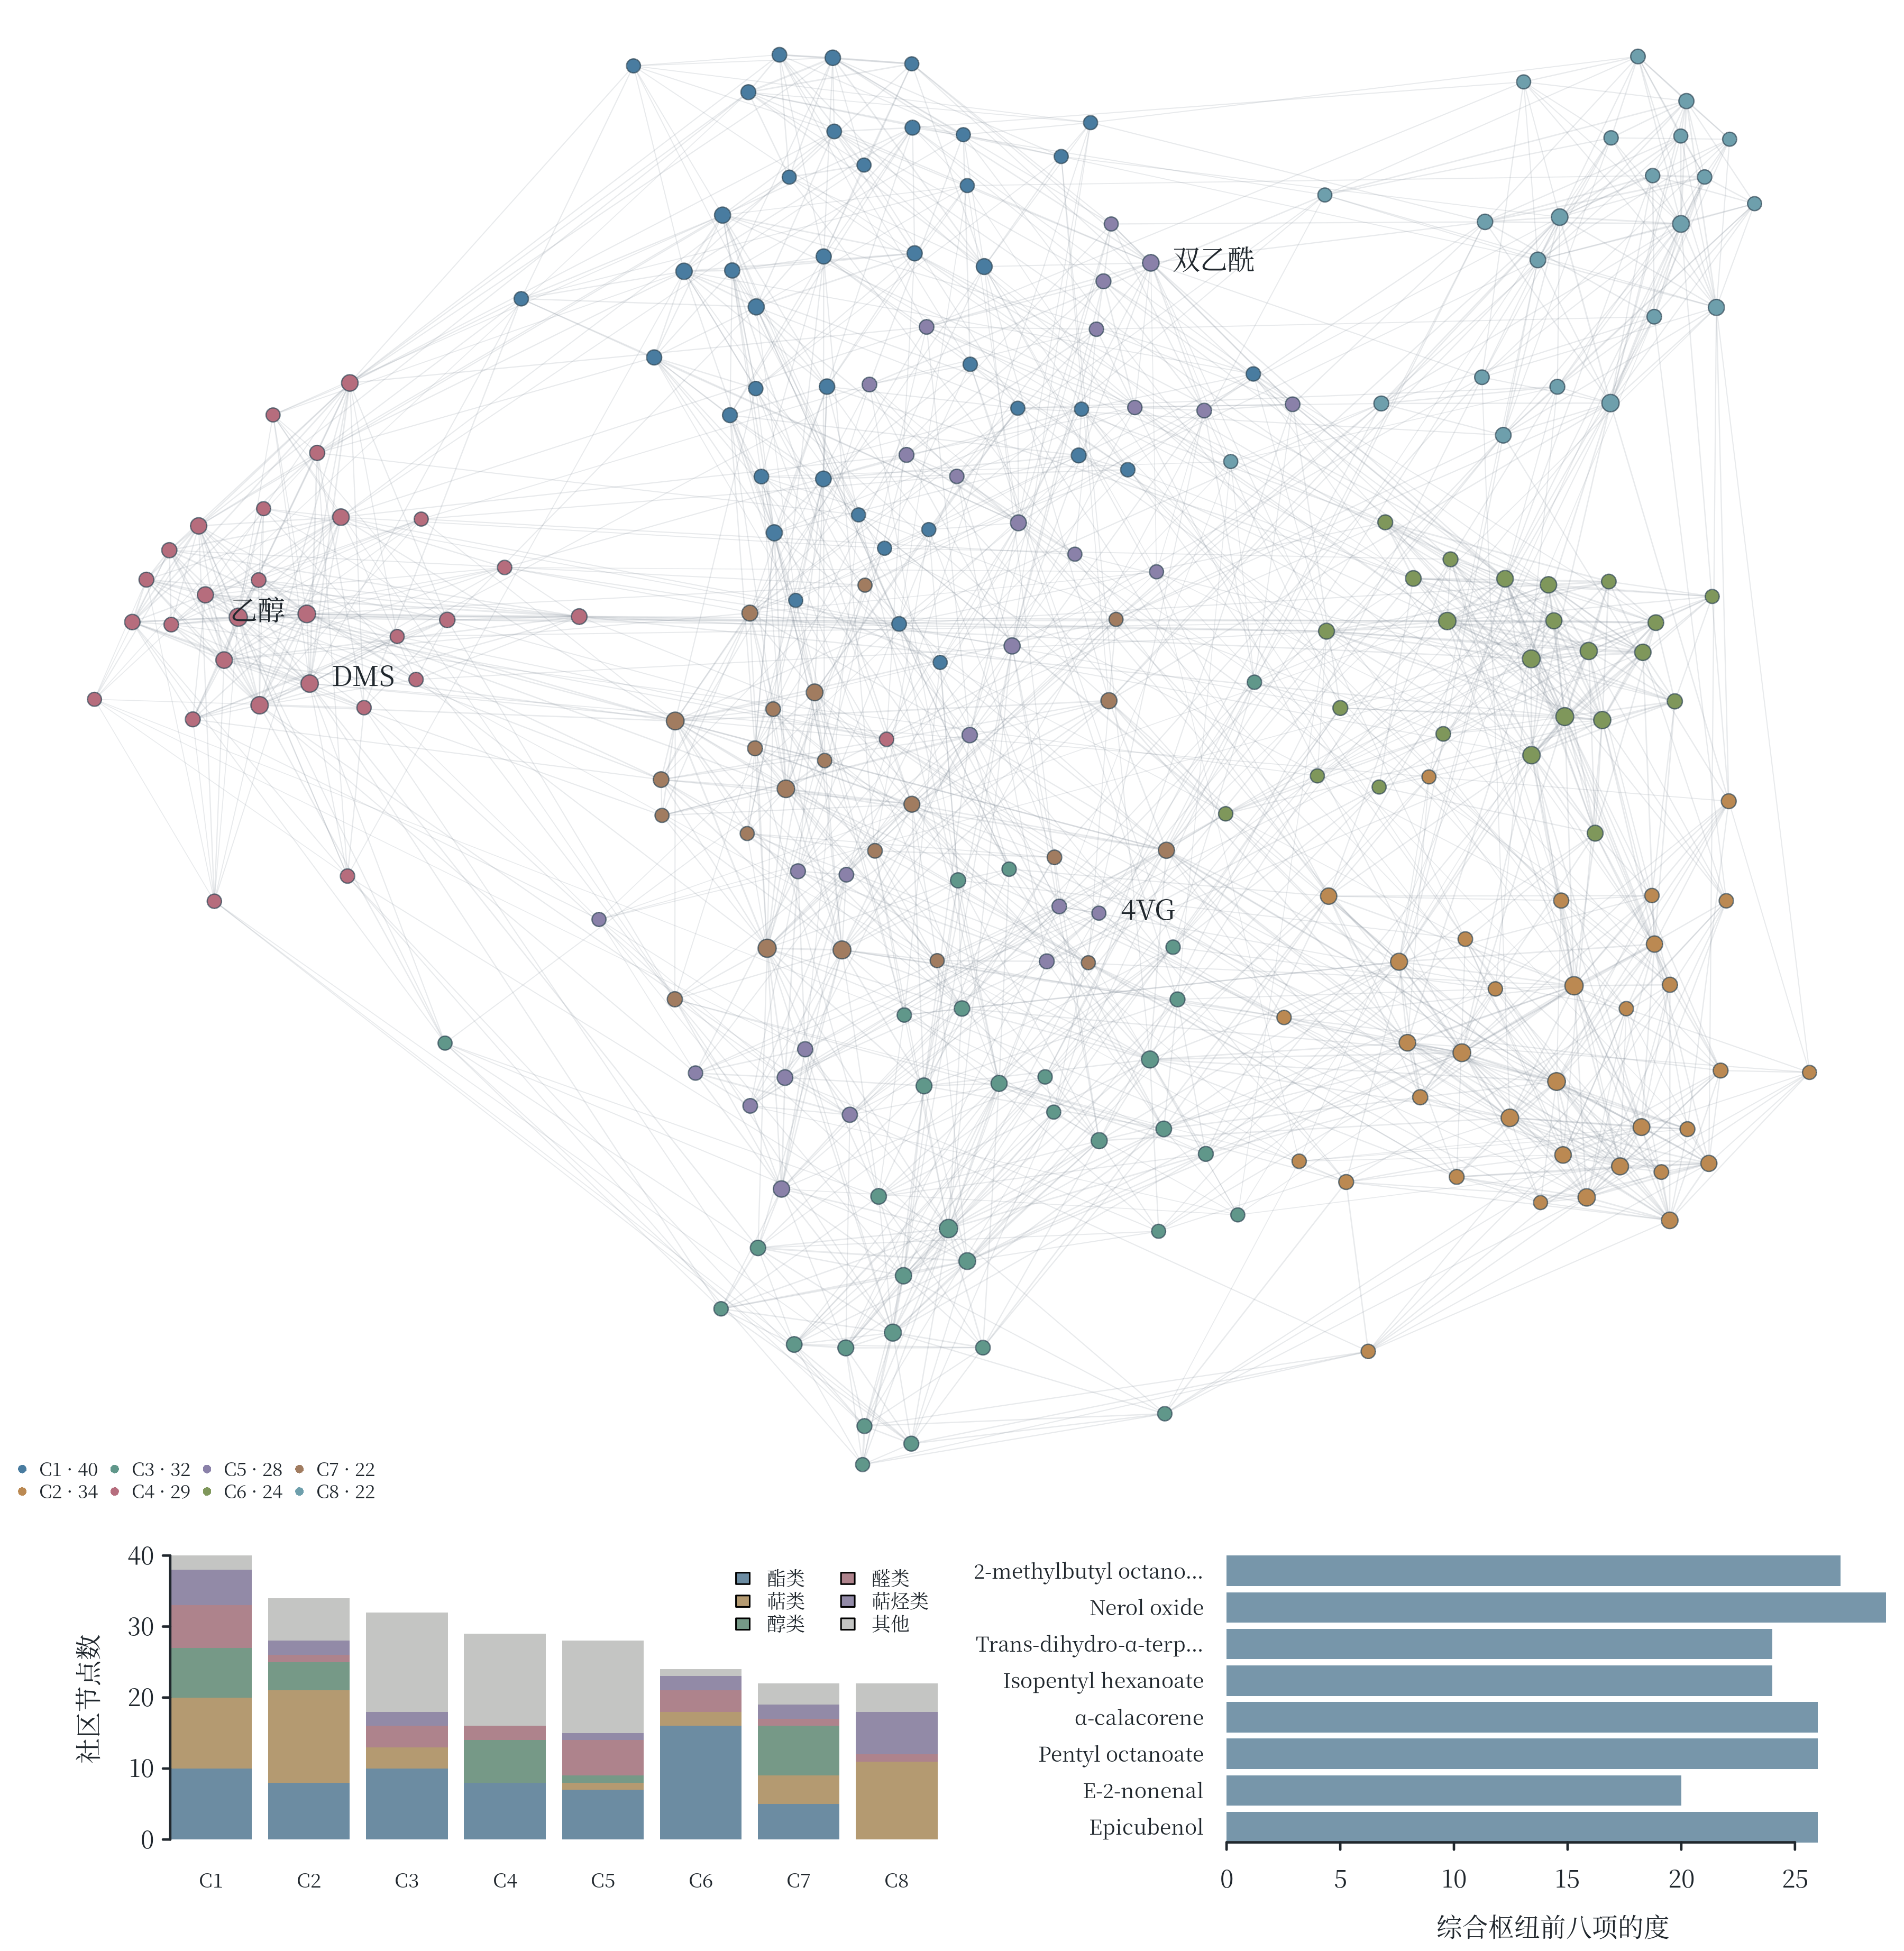
\includegraphics[width=\textwidth]{fig05_network.png}
  \caption{231 个节点的化合物关联网络。节点颜色表示 Louvain 社区，C1--C8 按社区规模降序编号，图例数字为节点数；节点大小表示度，布局为 ForceAtlas2。构图使用绝对相关，正负关联均可能成边，同社区不表示浓度同向变化，也不表示存在因果关系。}
  \label{fig:q2net}
\end{figure}


\subsubsection{五类排序与融合}

对感官维度 $s$ 比较五类排序：A 为绝对 Spearman 边际关联，逐维做 BH 多重检验校正；B 为标准化弹性网的绝对系数；C 为 ExtraTrees 的不纯度重要性；D 为 LightGBM 在训练样本上的平均绝对 SHAP 值\cite{lundberg2017}；E 为图平滑后的关联。D 是拟合内的描述性归因，不是独立留出的 SHAP；C 与 D 在相关特征之间的分摊与替代，不能解释成唯一的化学贡献。

弹性网使用插补、标准化与估计器组成的完整 Pipeline，内部 3 折按原始酒样编号分组，避免重采样得到的同款酒副本跨越内部训练与验证。ExtraTrees 固定 100 棵、最小叶样本 3，LightGBM 固定 100 棵，点估计与重采样使用完全相同的预算。

图平滑 E 并不是求解拉普拉斯惩罚回归。令 $S$ 为有符号边际相关矩阵、$W$ 为 $A$ 的行归一化矩阵，则
\begin{equation}
S_{E}=(1-\lambda)S+\lambda WS,\qquad \lambda=0.3,
\label{eq:smooth}
\end{equation}
再按绝对值排序。这是一跳加权平均，不是 $(I+\lambda L)^{-1}$；符号相反的邻居可以互相抵消，因此共享网络结构并不保证提升关键性辨识。

各方法把分数降序转为含平均并列秩的 $r^{(\nu)}_{j,s}$，用 Borda 平均秩融合：
\begin{equation}
\bar r_{j,s}=\frac{1}{5}\sum_{\nu\in\{A,B,C,D,E\}}r^{(\nu)}_{j,s}.
\label{eq:borda}
\end{equation}
候选按 $\bar r$ 升序截取，出现并列时按固定特征顺序确定。平均秩避免不同归因量纲直接相加，但方法之间相关，也没有“等权最优”的定理；本文把它当作透明的折中，并保留去网络与纯边际关联两个基线。

\subsubsection{重采样与选择稳定性}

以 250 款酒为单位有放回重采样 500 次，全部方法重新拟合：中位数插补、标准化与弹性网选参都重新执行，而不是复用点估计的中间结果。主化学候选的稳定性即式~\eqref{eq:freq}。

\subsection{实验设置}

弹性网网格为惩罚强度 0.03、0.1、0.3 与 $l_1$ 比例 0.3、0.7，每次重采样重新选参；图平滑系数固定 0.3；社区划分用加权 Louvain；重采样 500 次，随机种子 42。用途检查另做 5 折训练内 Top-3 选择，再对选中的 3 个变量训练固定强度 10 的 Ridge 并评价留出响应，所有目标等权汇总。

\subsection{结果与分析}

主化学候选共 150 项（50 个感官目标乘 3 项），平均入选频率 0.4332、中位数 0.3460，其中 19 项达到 0.8。全 231 指标诊断表对应的均值为 0.5105；排除理化与派生代理后稳定性明显下降，这一点必须如实报告，不能只引用诊断表的较高数字。

方法之间的一致性同样有限：全指标口径下五方法两两 Top-3 的 Jaccard 平均为 0.2870，说明共线替代与方法分歧仍然显著，不能写成“高度一致”。

表~\ref{tab:q2-top3} 给出 6 个代表性维度的化学候选与入选频率。4VG 维度的直接测量项最稳定（0.992），而双乙酰、DMS 与反式-2-壬烯醛都没有选出同名直接化合物：双乙酰的前三项是 pentyl octanoate、$\beta$-phellandrene 与 ethyl decanoate，频率约 0.390、0.336 与 0.350。这些至多是统计伴随物，不能取代对双乙酰的直接监测。

\begin{table}[H]
  \centering
  \caption{代表性感官维度的化学候选与 500 次重采样入选频率}
  \label{tab:q2-top3}
  \small
  \begin{tabularx}{\textwidth}{@{}l >{\hsize=1.2\hsize\raggedright\arraybackslash}X >{\hsize=0.8\hsize\raggedright\arraybackslash}X@{}}
    \toprule
    感官维度 & 化学候选（按主表顺序） & 入选频率 \\
    \midrule
    \file{A\_malt\_all} & $\beta$-phellandrene；ethyl linalool；5-methylfurfural & 0.452 / 0.222 / 0.142 \\
    \file{A\_hops\_citrus} & cis-dihydro-$\beta$-terpineol；methyl heptenone；geraniol & 0.492 / 0.336 / 0.280 \\
    \file{diacetyl} & pentyl octanoate；$\beta$-phellandrene；ethyl decanoate & 0.390 / 0.336 / 0.350 \\
    \file{dms} & sulfur dioxide；Z-dihydro-apofarnesal；terpinen-4-ol & 0.288 / 0.102 / 0.168 \\
    \file{X4vg} & 4-vinylguaiacol；neryl formate；4-ethyl-guaiacol & 0.992 / 0.294 / 0.194 \\
    \file{t2n} & glycerol；geraniol；$\beta$-phellandrene & 0.378 / 0.090 / 0.218 \\
    \bottomrule
  \end{tabularx}
  \par\vspace{3pt}
  \begin{minipage}{\textwidth}
    \footnotesize 注：候选按五法平均秩 $\bar r_{j,s}$ 升序排列，末列入选频率 $\hat\pi_{j,s}$ 为 500 次重采样的附带信息。两者口径不同，频率不随名次单调下降。
  \end{minipage}
\end{table}

图~\ref{fig:q2top3} 固定展示三类香气与五类缺陷共 8 个维度，其中在表~\ref{tab:q2-top3} 之外的两项用于补足香气与缺陷的覆盖；图中出现五个缺陷维度，不等于五类缺陷已获控制。

预测用途检查的结果不支持“网络不可替代”的说法：全指标边际、五法融合、去网络四法融合的
平均 $R^2$ 分别为 0.1170、0.1308、0.1312，去掉网络平滑反而略高；化学候选限定的结果
为 $R^2=0.0760$、$\mathrm{RMSE}=0.5166$。因此现有证据支持把网络用于结构展示与候选扩展，
不支持声称它带来已证实的性能提升。

网络构造的敏感性也直接对照 Top-3 集合：与 Top-10、平滑 0.3 相比，Top-5/0.3 
与硬阈值/0.3 的平均 Jaccard 约为 0.93 与 0.92，Top-10 平滑 0 与 0.6 约为 0.92 与 0.84。
这一诊断只针对全指标融合，不与主化学候选的频率混称；社区划分的调整兰德指数不能替代 Top-3 
敏感性。
\begin{figure}[H]
  \centering
  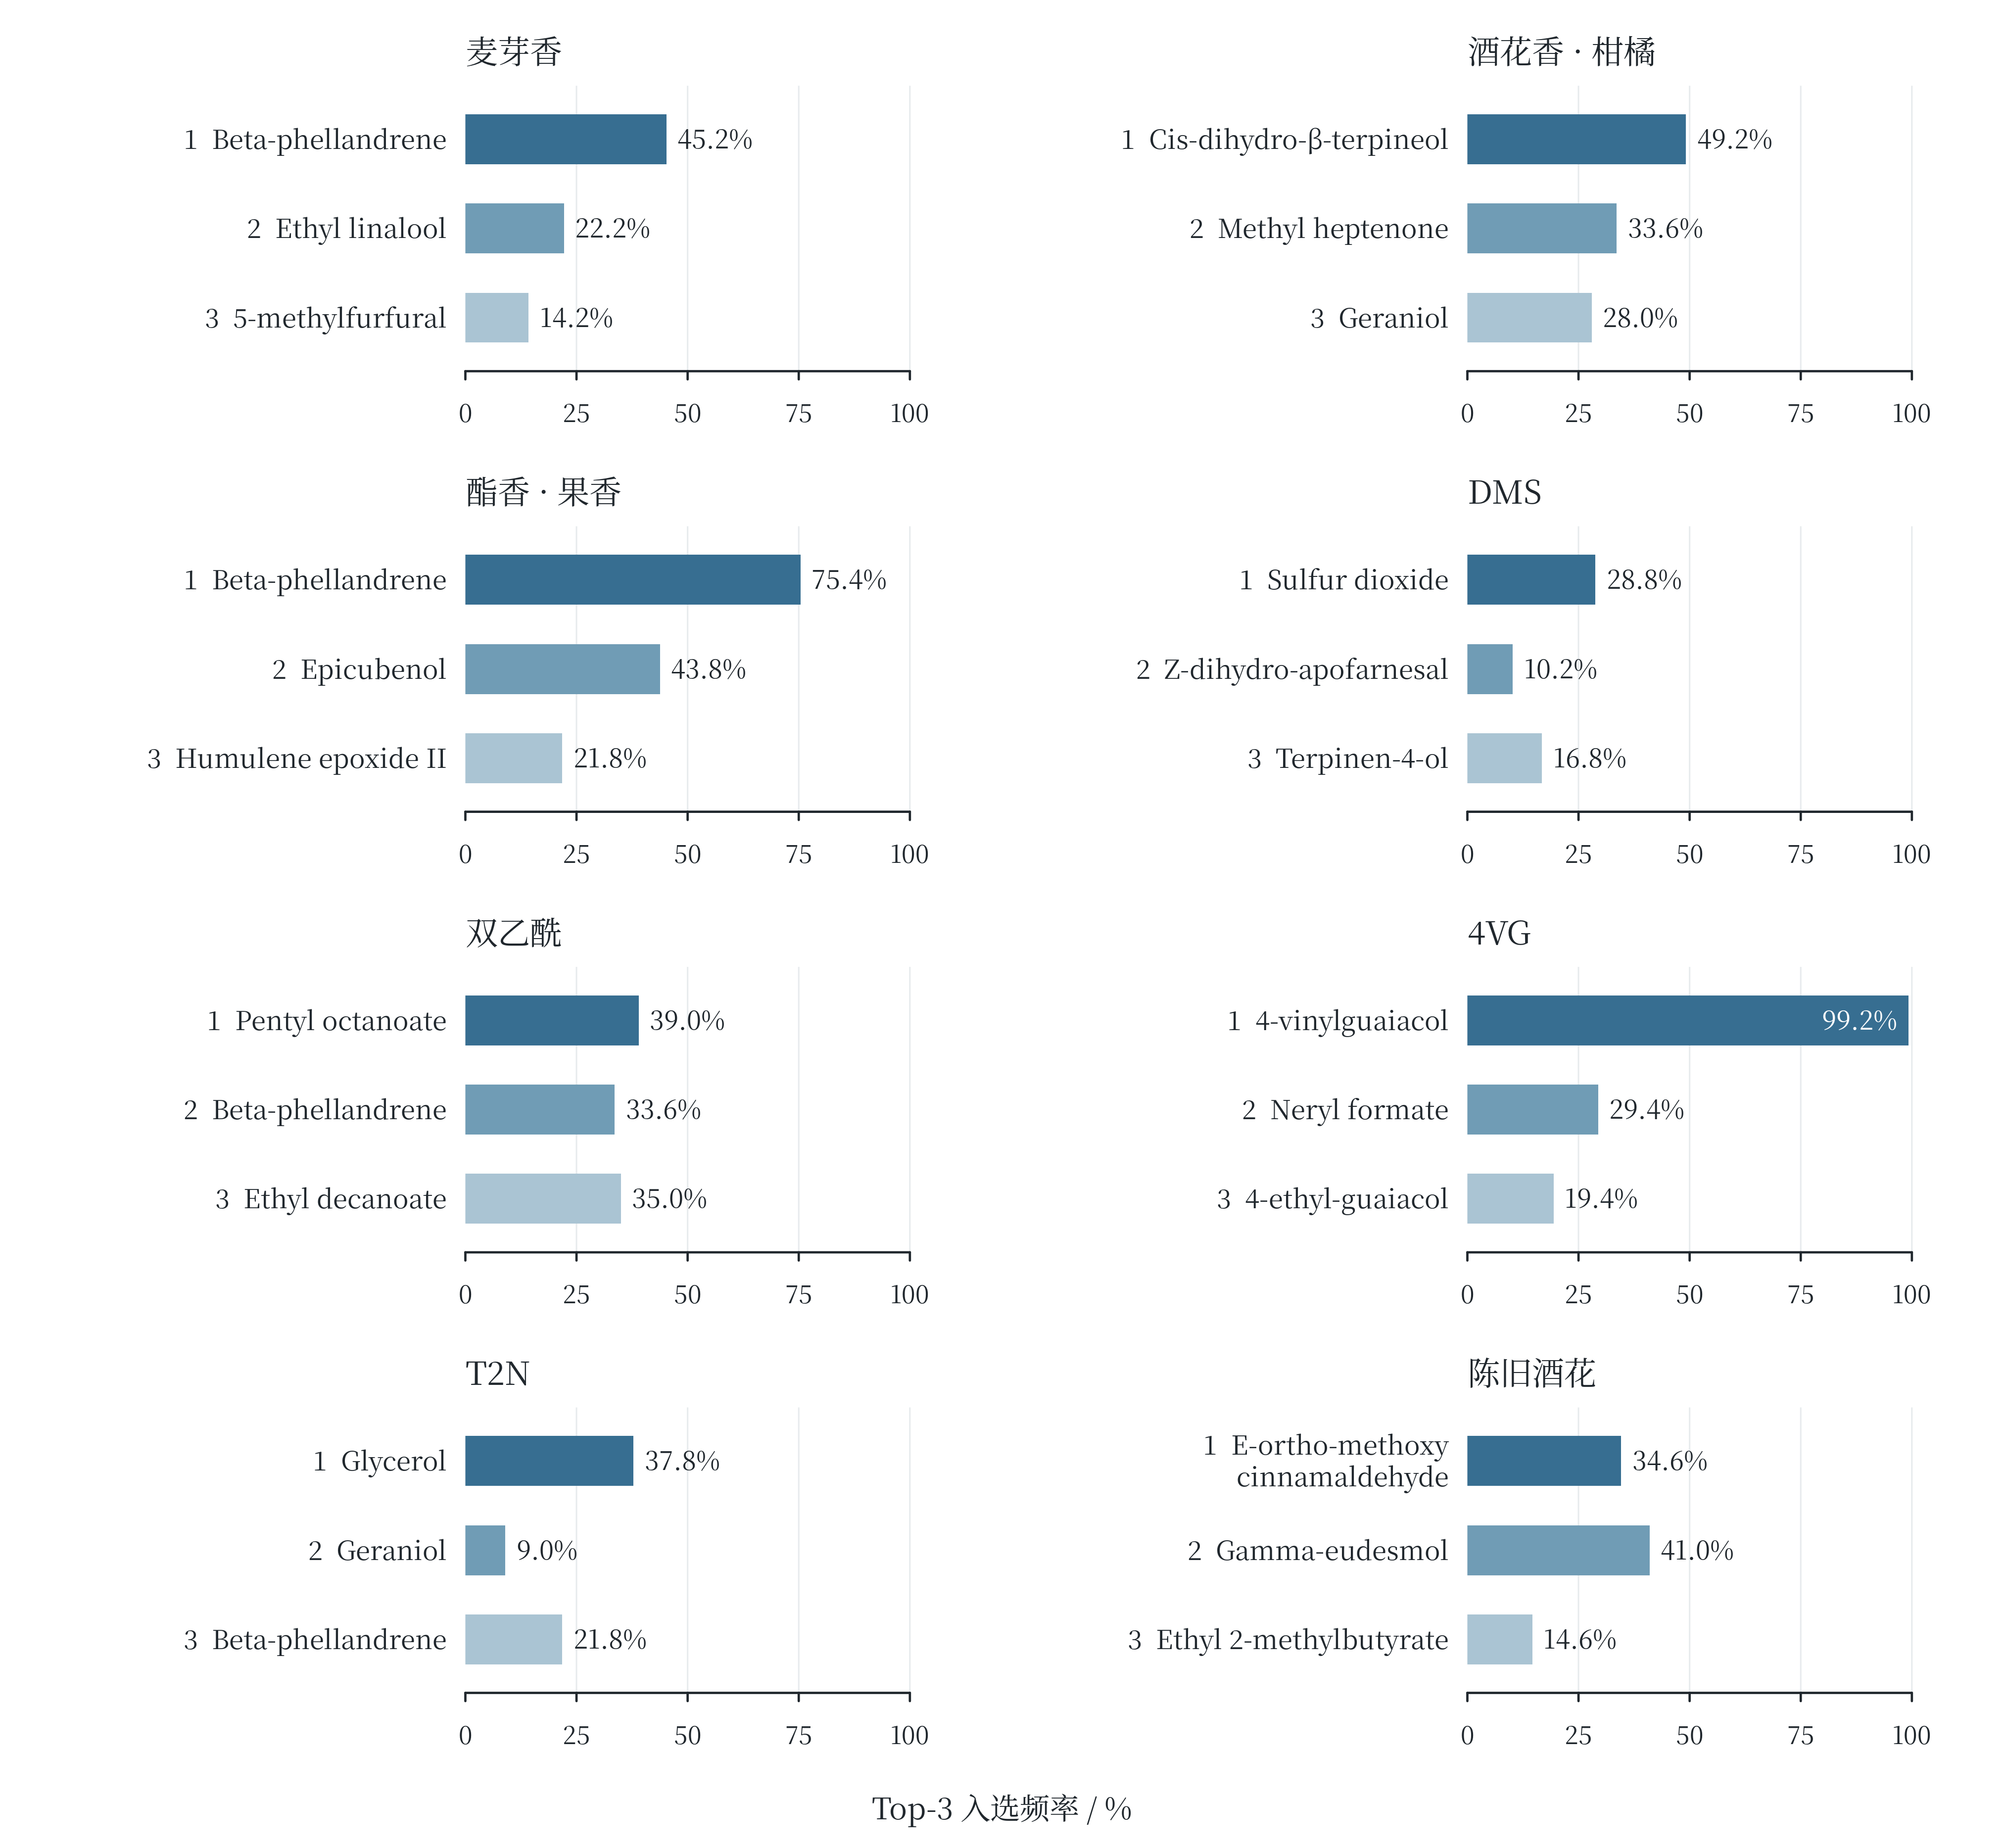
\includegraphics[width=\textwidth]{fig18_top3.png}
  \caption{八个代表性感官维度的 24 项化学候选。条目顺序为五法平均秩，柱长为 500 次酒样 bootstrap 下的 Top-3 入选频率；两者口径不同，频率不随名次单调下降。维度固定在三类香气与五类缺陷，未按结果好坏挑选。完整 50 维、150 项见附录。}
  \label{fig:q2top3}
\end{figure}


\subsection{化学合理性与先验敏感性}

\file{6.csv} 是 44 个化学与理化指标对 50 个感官属性的同源相关表，与边际关联的重合主要证明名称映射与计算一致，不构成外部泛化验证。富集检验（Fisher 检验加 BH 校正）用于描述候选的类别分布，其显著计数是“目标乘类别”的组合数，不能直接写成“多少种化学类别”。

另对全指标排名设置固定的文献知识分值 $p_{j,s}$：直接同名取 1、具体关联标志取 0.7、宽泛家族取 0.4、理化代理取 0.3、其余取 0，比较
\begin{equation}
u_{j,s}=1-\frac{\bar r_{j,s}-1}{230},\qquad u^{*}_{j,s}=u_{j,s}+\gamma p_{j,s},\quad\gamma\in\{0,0.1,0.2,0.5\}.
\label{eq:prior}
\end{equation}
该规则是机理先验的敏感性分析，不是由数据验证出的最优权重。每个 $\gamma$ 都在 500 次重采样内重做对应选择、计算自己的入选频率，不能沿用纯数据规则下的频率代替。$\gamma=0.5$ 时平均频率约 0.6412、与纯数据 Top-3 的重合约 0.4267；先验越强可能机械地越稳定，不能据此认定更接近真相。该情景也没有让所有同名物质回到 Top-3：双乙酰就不满足。

\subsection{讨论}

本数据下“简单边际基线、多方法候选、重采样与机理审查”的路线是合理的，但无法证明某一组 Top-3 就是最优或唯一。若要识别直接风味驱动，需要风格内条件分析与替代特征簇的条件置换；若要因果判断，还需外部或干预证据。

更复杂的图神经网络、深度归因或知识强制排序，目前没有在本文数据上显示出已验证的改进，因此不作为结论提出。

% ==================== 5 问题三 ====================
\section{问题三：风格条件生成与缺陷约束迁移}
\label{sec:q3}

\subsection{问题分析}

以风格为条件，本文在 70 个校准化学与理化指标上生成化合物谱，并由训练得到的感官代理给出标准化响应画像。需要先声明三条信息边界：输出是校准子谱，不是完整的 231 维化学谱；画像是模型代理的预测，不是实测评分；统计映射不等于可直接实施的酿造配方。

生成目标要兼顾风格分布与合理变异；迁移还需声明“相对源样本的缺陷约束”。在没有配对迁移实验时，源与目标两个分布并不能唯一识别真实的化学变化路径，本文的映射只是明确代价下的建模选择。

评价必须独立于拟合过程：生成参数只在训练部分估计，分布距离在留出样本上计算；感官画像的参照取留出实测评分的逐维中位数，而不是同一批模型输出的拟合值。

\subsection{评价指标}

分布距离采用 RBF 核 MMD 平方的去对角 U 统计量，核宽由目标风格的训练距离确定；有限样本估计可为负，不截断为零。覆盖度定义为留出真实样本至少落入一个生成邻域的比例，邻域半径由目标训练样本留一最近邻距离的中位数确定。风格保真用只在训练样本上拟合的随机森林分类器，同时报告它在真实留出集上的准确率，以免把生成样本上的高命中率当作泛化能力。画像误差以留出实测评分的逐维中位数为参照，报告 RMSE。

精确度、画像 Pearson 相关与马氏距离同样按上述划分计算。精确度与覆盖度虽然都是比例，但分母不同——覆盖度以留出真实样本为分母，精确度以每轮设定的生成条数为分母，后者随生成规模改变，两者并列会误导；画像 Pearson 相关与马氏距离亦不与 RMSE 同尺度。因此这四项随结果文件提供，不进入表~\ref{tab:q3-res}。

分别记录各风格，再对三个风格等权平均、对 5 次重复汇总。需要说明，重复留出的样本相互重叠，其标准差不是独立实验的置信区间。

\subsection{模型构建：从基线到正确的高斯最优传输}

\subsubsection{基线与条件 copula}

最简单的条件基线是同风格经验行重采样：它保留已见样本，却不能提供“生成新样本”的证明。另比较风格均值加独立噪声，以及风格均值加共享协方差噪声：
\begin{equation}
\tilde z=\mu_g+\operatorname{diag}(\sigma_g)\epsilon,\qquad
\tilde z=\mu_g+\Sigma_w^{1/2}\epsilon,\qquad \epsilon\sim N(0,I),
\label{eq:noise-baseline}
\end{equation}
其中共享协方差 $\Sigma_w$ 由训练样本先减去各自风格均值后的残差估计，避免把风格中心之间的差异当成风格内部波动。

主候选为条件 Gaussian copula。对训练风格 $g$ 的每列计算平均并列秩 $r_{i,j}$，构造有限正态分数
\begin{equation}
u_{i,j}=\Phi^{-1}\left(\frac{r_{i,j}-1/2}{n_g}\right),
\label{eq:normal-score}
\end{equation}
由风格内正态分数估计 Ledoit--Wolf 相关矩阵，再向共享的风格内相关结构收缩：
\begin{equation}
R_g=(1-\lambda_g)\hat R_g+\lambda_g R_w,\qquad \lambda_g=\frac{n_0}{n_0+n_g},\quad n_0=20.
\label{eq:shrinkage}
\end{equation}
采样 $v\sim N(0,R_g)$，再用训练风格的经验分位数函数 $Q_{g,j}$ 逆映射：
\begin{equation}
\tilde c_j=Q_{g,j}\left(\Phi(v_j)\right).
\label{eq:copula}
\end{equation}
该方法以简单的相关结构控制小样本方差，但边际正态化并不推出真实联合高斯，经验边际也不能可靠推断训练范围之外的尾部；零值与检出限并列直接进入混合经验分布，不在采样后重复强制置零。$n_0=20$ 是预设的收缩强度，本文另比较 5 与 50，不称 20 为已证最优。

\subsubsection{协方差匹配与正确的高斯最优传输}

令 $\Sigma_s,\Sigma_t$ 为源与目标的正定收缩协方差。白化—着色映射
\begin{equation}
A_{\mathrm{WC}}=\Sigma_t^{1/2}\Sigma_s^{-1/2}
\label{eq:wc}
\end{equation}
能匹配高斯矩，但在平方欧氏代价下一般不是最优传输。正确的高斯 $W_2$ 映射\cite{peyre2019}为
\begin{equation}
A_{\mathrm{OT}}=\Sigma_s^{-1/2}\left(\Sigma_s^{1/2}\Sigma_t\Sigma_s^{1/2}\right)^{1/2}\Sigma_s^{-1/2},\qquad
T(z)=\mu_t+A_{\mathrm{OT}}\left(z-\mu_s\right),
\label{eq:ot}
\end{equation}
矩阵平方根通过对称特征分解获得，必要时加小的正定修正。两式含义不同：白化—着色映射只匹配矩，高斯 $W_2$ 映射才在平方代价下最优，因此分别给出、分别报告，不把两者的数值混用。

生成支路从其他风格的中心化训练残差池抽样，分别做协方差匹配或高斯 OT；另把 OT 后逐列对齐目标训练经验分位数作为独立对照。秩校准只用于该生成对照，Pils/Lager 到 Tripel 的逐酒迁移不附加这一步。分位数映射与缺陷投影都可能破坏原始映射的最优性质，因此不把整条后处理链称为全局最优传输。

\subsection{缺陷不恶化的操作定义}

设 $c_s$ 为源样本某缺陷列的数值，$c$ 为迁移后的数值，$\tau$ 为声明情景下的感官阈值。按题目所列的超阈值项，主迁移要求超阈值程度不增加：
\begin{equation}
\left(c-\tau\right)_{+}\le\left(c_s-\tau\right)_{+},\qquad\text{等价于}\quad c\le\max\left(\tau,c_s\right).
\label{eq:defect-main}
\end{equation}
更保守的 strict 对照同时要求浓度不增加且不超过阈值：
\begin{equation}
c\le\min\left(\tau,c_s\right).
\label{eq:defect-strict}
\end{equation}
另保留按目标风格 $\max(\tau,q_{75})$ 截断的 style 对照，但它不保证相对源样本不恶化，因此不能替代主约束。投影后的零违反率只证明实现满足所选约束，不是独立的分布质量证据。

DMS、双乙酰、4VG 的情景上限分别取 17.25、0.09、0.10，统一使用校准表的相应单位；它们都是本研究中的感官约束，不是食品安全限值或法规标准。

反式-2-壬烯醛的单位有两种可能解读：按 mg/L 与按 $\mu$g/L，二者相差 $10^{3}$ 倍，附件中没有足以判定哪一侧正确的校准记录。由于 $0.10\ \mu\mathrm{g/L}=0.00010\ \mathrm{mg/L}$，本文以保留附件标注、上限取 0.00010 为主情景，另报告按 $\mu$g/L 解释、上限取 0.10 的替代情景，约束与超阈值评价分别计算。

stale hops 不是单一化合物。用若干列标准化均值构造代理、并要求迁移后不升高，缺少机理依据与预测验证，还会连带压低本应上升的果香酯类；因此本文不对它施加化学列约束，只报告独立感官代理对 stale hops 的预测变化及其留出能力，不声称真实缺陷已获保证。

\subsection{实验设置}

从随机种子 42 起，重复 5 次按风格留出约 20\% 的样本：每轮 191 个训练、59 个留出，每个风格至少有 1 个留出与 2 个训练样本；Tripel、Kriek、Lambic 每轮的留出样本数分别为 6、2、3。经验边际、阈值上限、核宽与协方差都只由训练部分估计。感官代理在训练部分用内部 3 折比较 Ridge 与 PLS 并选参，再预测留出实测响应。

完成独立留出评价之后，才用全部 250 款酒重拟合，输出三个风格各模型 300 条谱及连续感官代理画像。该全量拟合只用于最终描述性产物，不计为独立验证。

\subsection{结果与分析}

独立留出下的对照结果见表~\ref{tab:q3-res}。数值为三风格等权平均，再对 5 次重复平均。

\begin{table}[H]
  \centering
  \caption{独立留出真实参照下各生成方法的对照（三风格等权、5 次重复平均）}
  \label{tab:q3-res}
  \small
  \begin{tabularx}{\textwidth}{@{}>{\raggedright\arraybackslash}X c c c c@{}}
    \toprule
    方法 & $\mathrm{MMD}^{2}$ & 覆盖度 & 分类命中率 & 实测画像 RMSE \\
    \midrule
    经验行重采样 & 0.0532 & 0.5333 & 1.0000 & 0.2913 \\
    独立噪声 & 0.0498 & 0.4556 & 0.9376 & 0.2979 \\
    共享协方差 & 0.0494 & 0.6000 & 0.9027 & 0.2970 \\
    条件 copula & 0.0445 & 0.7444 & 0.9962 & 0.2919 \\
    协方差匹配 & 0.0450 & 0.6778 & 0.9313 & 0.2938 \\
    高斯 OT & 0.0446 & 0.7111 & 0.9313 & 0.2937 \\
    OT 加目标边际 & 0.0427 & 0.7333 & 0.9927 & 0.2913 \\
    OT 加边际加 style 上限 & 0.0430 & 0.7333 & 0.9936 & 0.2908 \\
    \bottomrule
  \end{tabularx}
  \par\vspace{3pt}
  \begin{minipage}{\textwidth}
    \footnotesize 注：本表只并列展示各方法的量级，不对任何一列标注最优。理由见正文：$\mathrm{MMD}^{2}$ 的方法间极差 0.0105 小于其重复间标准差 0.0569，实测画像 RMSE 的方法间极差 0.0071 小于其重复间标准差 0.0815；覆盖度与分类命中率未给出重复间区间。
  \end{minipage}
\end{table}

条件 copula 的 $\mathrm{MMD}^{2}$ 为 0.0445、覆盖度 0.7444、分类命中率 0.9962、实测画像 RMSE 为 0.2919。各方法的实测画像 RMSE 集中在 0.2908--0.2979、极差仅 0.0071，不存在 OT 链条大幅领先的证据。

表~\ref{tab:q3-res} 的并列差异不足以支撑任何一列的排序。八种方法的 $\mathrm{MMD}^{2}$ 覆盖 0.0427--0.0532，方法间极差 0.0105；而本节后文给出的重复间标准差为 0.0569，是方法间极差的 5.4 倍，五次重复均值本身的标准误约 $0.0569/\sqrt{5}\approx0.025$，仍是极差的 2.4 倍。实测画像 RMSE 的方法间极差 0.0071 同样远小于其重复间标准差 0.0815。$\mathrm{MMD}^{2}$ 的三风格等权均值 0.0445 还小于它自己的重复间标准差，而 5.2 节已说明该 U 统计量可为负，因此现有留出不足以判定生成分布与留出真实分布之间存在可分辨差异。覆盖度与分类命中率未给出重复间区间，按同一口径一并不作排序。

因此本文只把表~\ref{tab:q3-res} 用于并列展示各方法的量级，不对任何一列宣称“最好”。经验行重采样的生成分类命中率为 1.0000，却未取得最小的独立 $\mathrm{MMD}^{2}$，这正说明命中率不衡量生成质量。真实留出的分类准确率五轮均值约 0.5695，与合成样本上的高命中率不是同一对象。

copula 的 $\mathrm{MMD}^{2}$ 在 5 次重复间的标准差约 0.0569，画像 RMSE 的标准差约 0.0815，说明小留出集带来的波动很大。收缩强度 $n_0=5,20,50$ 的平均 $\mathrm{MMD}^{2}$ 约为 0.0448、0.0445、0.0443，差异不足以证明 20 最优。

感官代理每轮在训练内都选中 Ridge，留出宏平均 $R^2$ 约 0.2129；stale hops 单维的平均 $R^2=-0.0466$，因此它的迁移预测只能作弱诊断。留出集小、重复划分重叠且风格样本不均衡，这些结果不能外推到所有商业啤酒。

全量重拟合后的两个描述性产物见图~\ref{fig:q3pca} 与图~\ref{fig:q3radar}：前者是 70 维校准子谱的低维投影，后者是生成谱经感官代理后的核心画像。两者都不计为独立验证，生成质量的独立留出论证仍以表~\ref{tab:q3-res} 为准。

\begin{figure}[H]
  \centering
  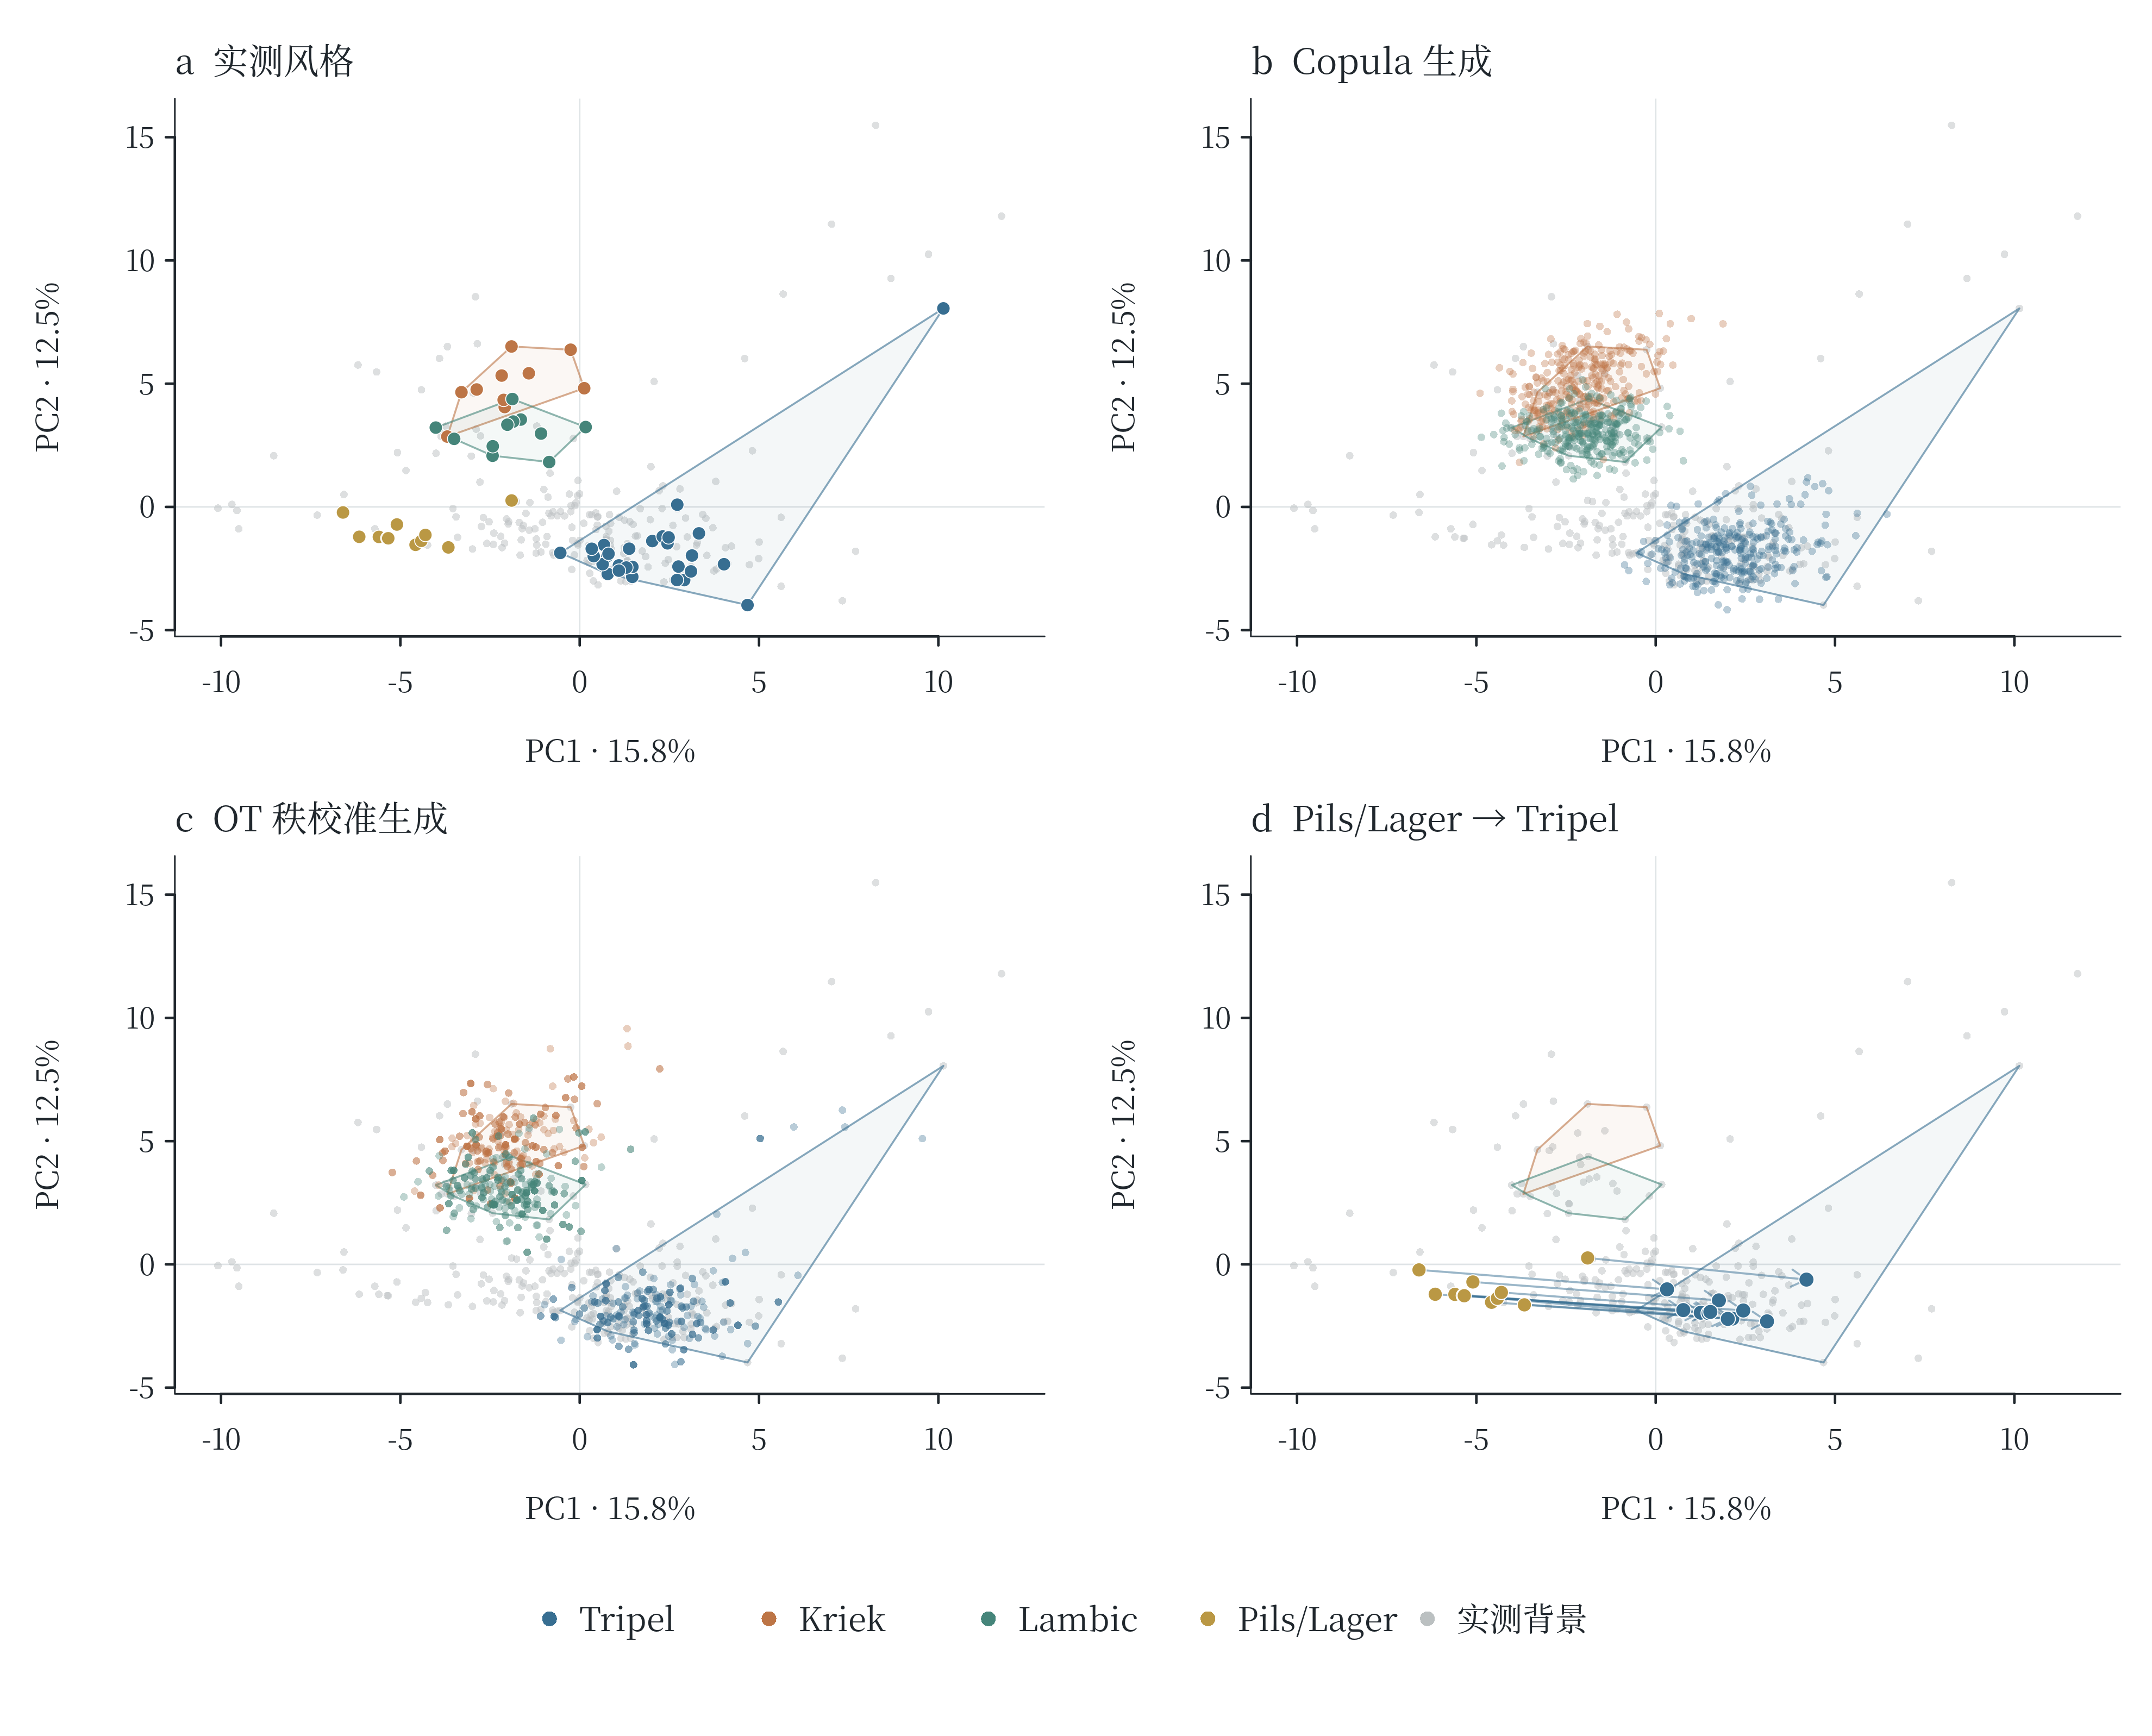
\includegraphics[width=0.75\textwidth]{fig19_pca.png}
  \caption{70 维校准子谱的 PCA 投影，坐标只在 250 款实测酒上拟合。(a) 实测；(b)(c) 三个风格各 300 条条件 copula 
  与高斯 OT 秩校准生成谱；(d) 11 款源酒到主约束迁移结果的配对箭头。PC1 约 15.8\%、PC2 约 12.5\%、合计约 28.3\%，}
  \label{fig:q3pca}
\end{figure}


\begin{figure}[H]
  \centering
  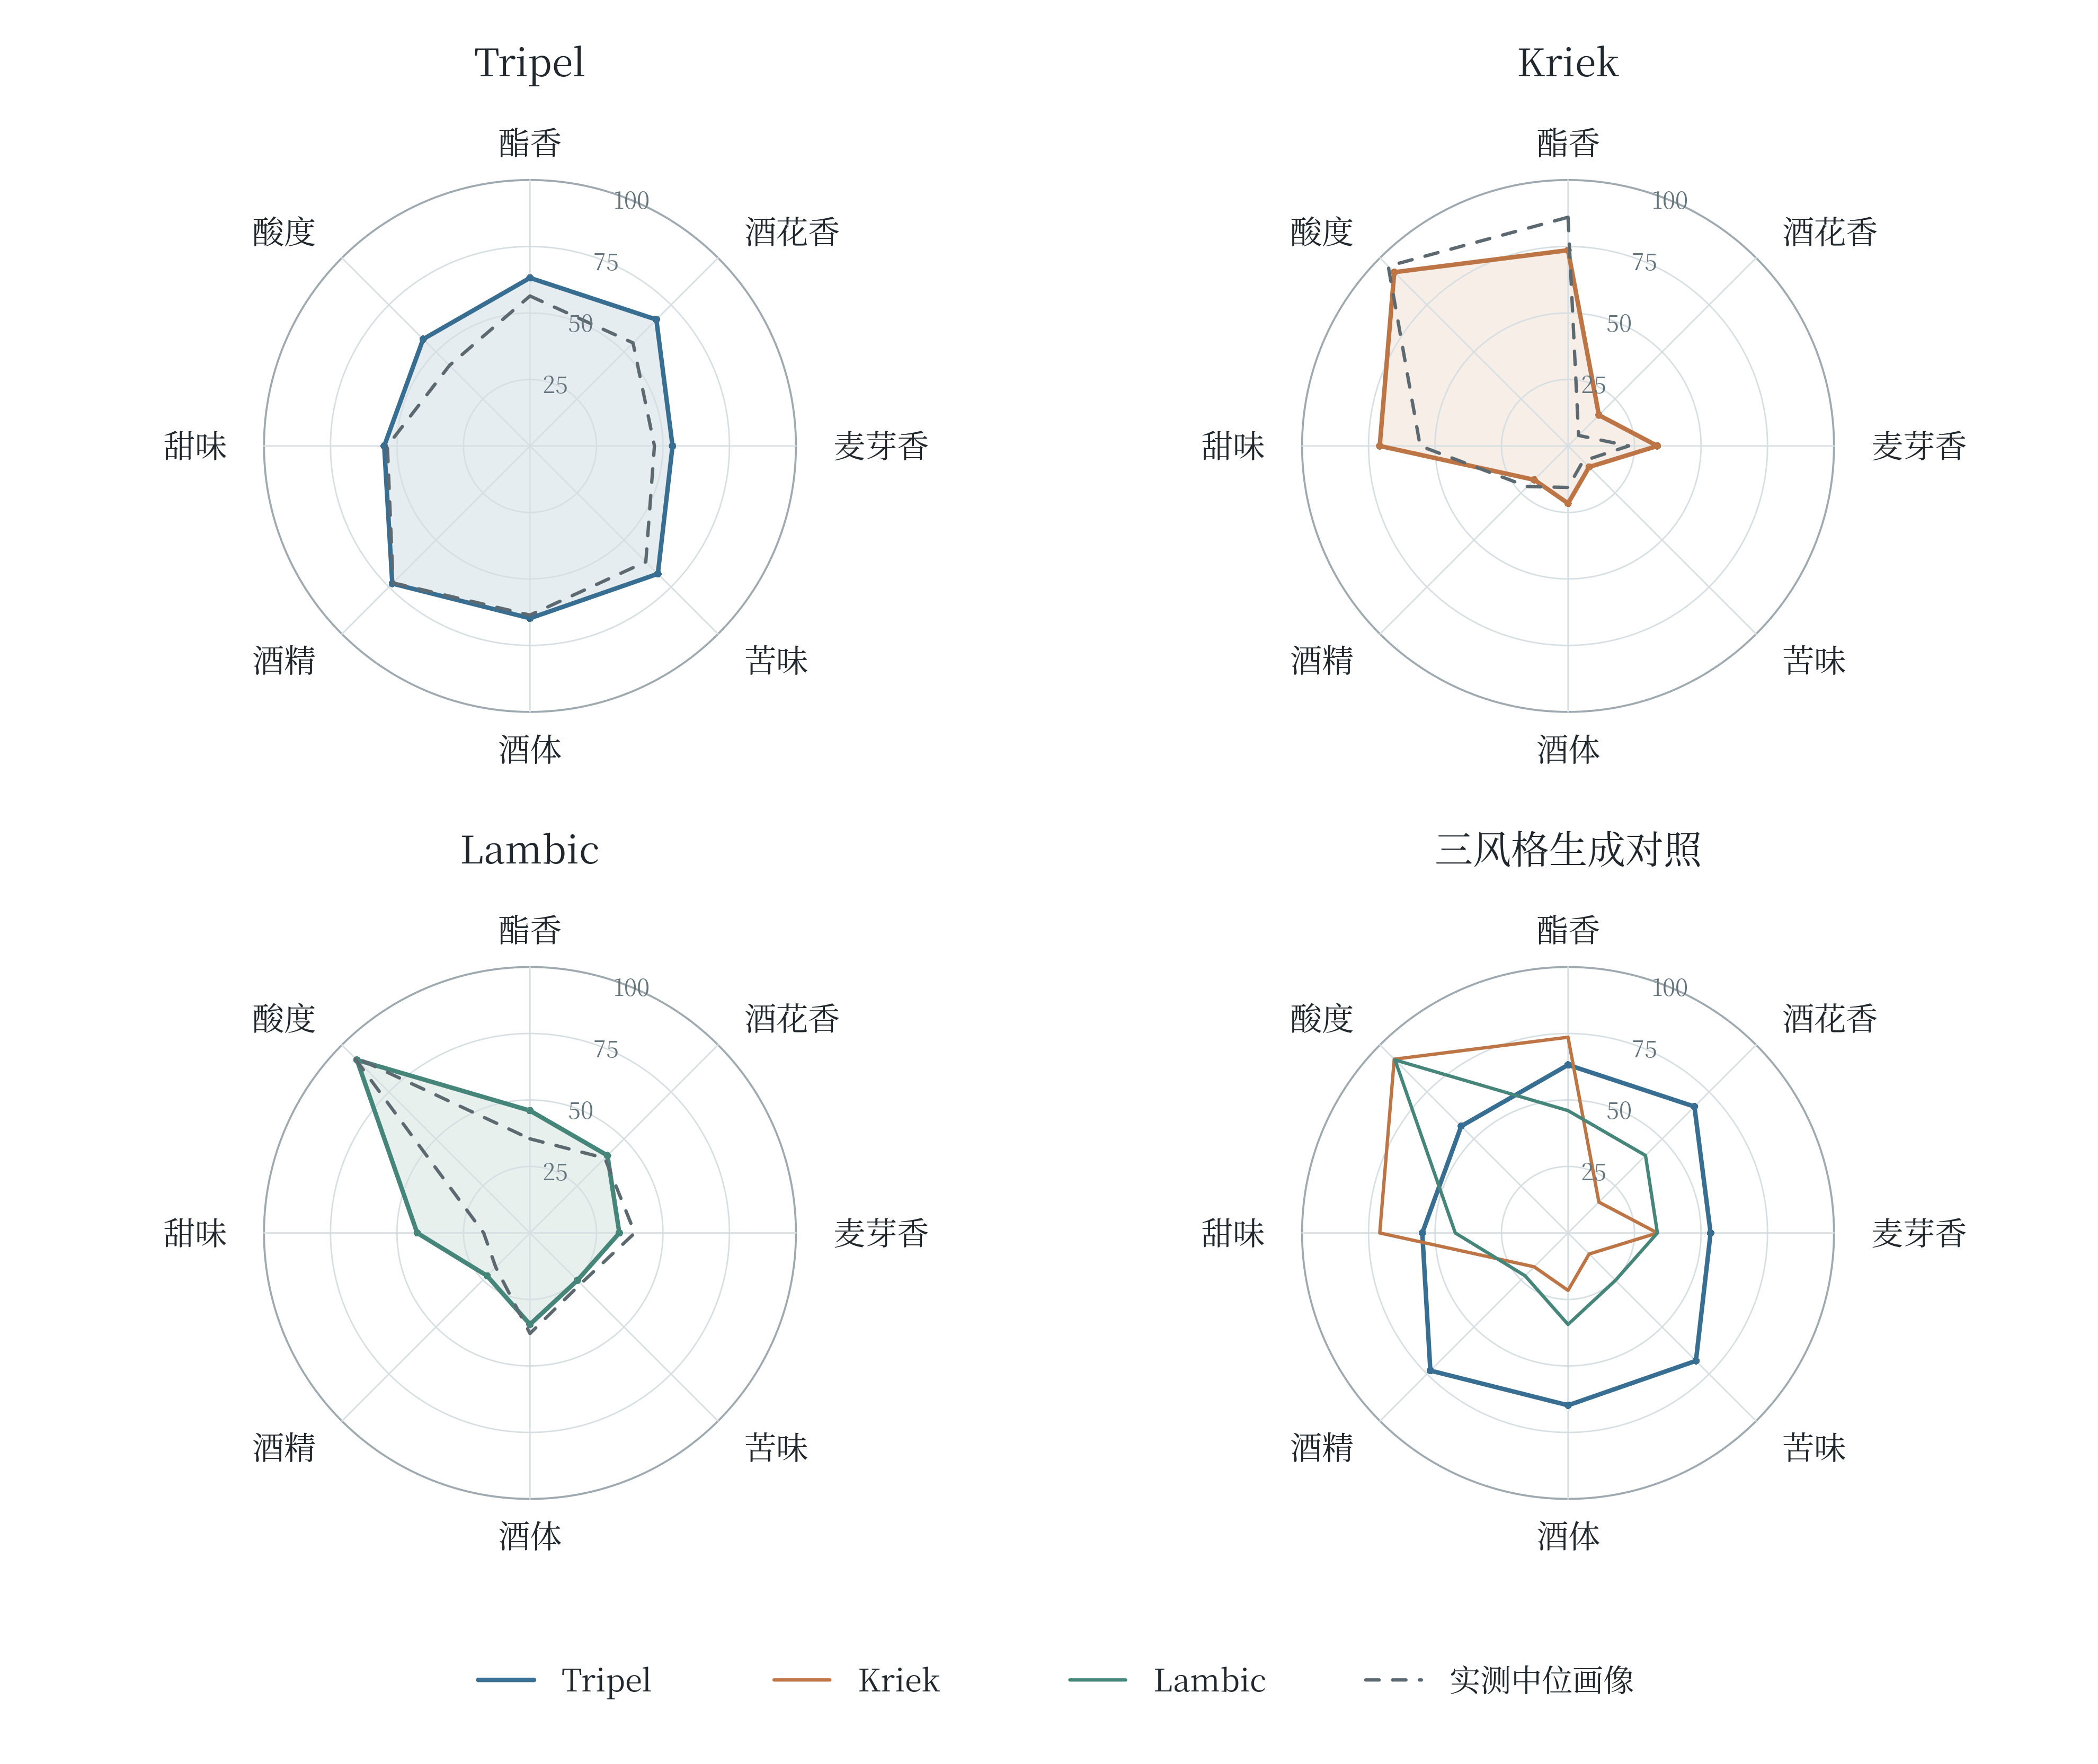
\includegraphics[width=0.75\textwidth]{fig20_radar.png}
  \caption{三个风格的生成与实测中位感官画像；第四面板叠加三风格生成画像。半径为统一实测参考下的感官响应百分位（0--100），
  曲线为组内中位响应的映射：50 表示处于全体实测响应的中间位置，100 表示高于全部该维度实测响应。八维依次为酯香、酒花香、麦芽香、苦味、酒体、酒精、甜味、酸度。}
  \label{fig:q3radar}
\end{figure}


\subsection{跨风格迁移结果}

Pils/Lager 到 Tripel 的 11 款源酒使用正确的高斯 OT 迁移。在两个单位情景下，主约束式~\eqref{eq:defect-main} 在四类直接化合物上均无恶化（0/11）；strict 更强约束下，浓度升高与超阈值率也均为 0。

相反，style 对照的 DMS 与双乙酰超阈值程度在 11 款源酒上全部升高（11/11），4VG 仅
1 款升高，反式-2-壬烯醛按附件单位时同样为 11/11、按替代单位时为 0/11（图~\ref{fig:q3trans}）。
因此 style 不能替代题目给出的主约束，反式-2-壬烯醛的单位选择还会直接改变这一具体结论
——这正是本文必须双情景报告的原因。

\figinsert[\textwidth]{fig21_transfer}{%
上方为感官代理画像，下方为四类直接化合物的超阈值恶化酒样数，两种反式-2-壬烯醛
单位情景分列。下方柱高为相对各自源酒超阈值程度 $\max(\mathrm{OAV}-1,0)$ 增加的酒样数，
不是超过阈值的总酒样数；0 表示在该情景与所用阈值下无对应数值恶化，不保证浓度均下降、
真实品评改善或工艺可达。}{fig:q3trans}

这些约束只对声明的四类化学指标成立。stale hops 没有可靠实测或代理保证；派生指标之间的一致性、工艺可达性与人的最终品评也未验证。本文把它们列为尚未解决的边界，而不是用高分类命中率代替验证。

\subsection{讨论}

条件 copula 是控制小样本估计方差的合理候选，正确的高斯 OT 是声明特征空间与平方代价下的迁移映射；两者都不是经证明的真实酿造机制。独立留出对照没有显示某个复杂后处理在全部指标上占优，高合成分类命中率也不能替代真实分布验证。

三个边界仍未解决。其一，完整复刻目标风格分布与所有样本满足缺陷约束在数学上可能冲突，简单截断还会在边界产生概率堆积，不等价于从可行区域的条件分布抽样。其二，反式-2-壬烯醛的单位需要原校准或测量文档确认，确认前保留双情景。其三，派生指标之间的代数一致性与实际工艺可行性需要单独的化学与工程核验。

\section{结论与建议}
\label{sec:conclusion}

\subsection{结论及方法选择}

问题一的高维小样本结构支持正则化、树模型与少参数融合的比较，但不自动支持深度模型或复杂权重优化。训练内选型流程的 15 折宏平均 $\bar R^2=0.2306$，化学特征相对仅用风格标签的均值基线仍提供预测增益；五模型平均略优于最强单体，两模型平均并未改善，堆叠也没有全面优势。预设的相对分级便于报告，但现有数据不能恢复人工绝对 0--6 量表，两项乙醛也不能补造监督标签。

问题二的网络描述与多方法筛选满足题目指定的分析路线，但关键候选并不唯一。化学限定主表的平均入选频率 0.4332、19/150 项达到 0.8；在固定线性读出器下，化学 Top-3 的 5 折宏平均 $R^2$ 仅 0.0760。全指标去网络对照没有降低预测表现，因此网络的价值目前主要是结构展示与候选扩展，不能宣称预测必要性或化学因果性。直接缺陷监测应优先核对同名物质与测量方法，而不是只监测统计代理。

问题三中，条件 copula 是控制小样本估计方差的合理候选，正确的高斯 OT 是声明特征空间与平方代价下的迁移映射，两者都不是经证明的真实酿造机制。独立留出对照没有显示某个复杂后处理在全部指标上占优，高合成分类命中率也不能替代真实分布验证。超阈值程度约束与 strict 对照能保证所声明的四类化合物的数值关系，却不能自动保证 \file{stale\_hops}、混合感知、配方平衡或实际酿造可行。

\subsection{局限与下一步验证}

绝对评分锚点与品评员处理规则缺失，应补充独立的原始 0--6 评分，再检验有序模型与校准。
161 个未校准特征的底数不能由模型表现倒推；反式-2-壬烯醛的单位需原校准或测量文档确认，
未确认前同时保留两种情景。共线化合物的直接作用需要风格内条件分析与外部或干预证据。
生成分布需要增加独立真实样本与人的感官验证，派生指标之间的代数一致性也应单独核验。

上述新增实验属于后续工作，未计入本文结果。外部评论词频仅能校验风格语义，
不能充当独立的逐酒感官标签。在实际应用中应将模型作为候选筛查工具，
通过化学检测与品评验证后再决定配方或工艺。

\begin{thebibliography}{99}
\raggedright
\zihao{5}
\setstretch{1.2}

\bibitem{liu2023}
刘倩，贾建华，白艳龙，等，啤酒风味物质及分析技术研究进展，中国酿造，42(8)：20-27，2023。

\bibitem{guguoxian}
顾国贤，酿造酒工艺学，第 2 版，北京：中国轻工业出版社，1996。

\bibitem{lijj2025}
李俊杰，刘智颖，赵丽娜，等，基于固相微萃取结合气相色谱-质谱联用技术分析苦荞啤酒中关键香气物质，中国酿造，44(7)：139-147，2025。

\bibitem{schreurs2024}
Schreurs M, Piampongsant S, Roncoroni M, et al., Predicting and improving complex beer flavor through machine learning, Nature Communications, 15: 2368, 2024.

\bibitem{cohen1968}
Cohen J, Weighted kappa: nominal scale agreement with provision for scaled disagreement or partial credit, Psychological Bulletin, 70(4): 213-220, 1968.

\bibitem{lihang}
李航，统计学习方法，第 2 版，北京：清华大学出版社，2019。

\bibitem{zhouzhihua}
周志华，机器学习，北京：清华大学出版社，2016。

\bibitem{wanghuiwen}
王惠文，偏最小二乘回归方法及其应用，北京：国防工业出版社，1999。

\bibitem{wangxiaofan}
汪小帆，李翔，陈关荣，复杂网络理论及其应用，北京：清华大学出版社，2006。

\bibitem{maosongsong}
茆诗松，程依明，濮晓龙，概率论与数理统计教程，第 3 版，北京：高等教育出版社，2019。

\bibitem{blondel2008}
Blondel V D, Guillaume J L, Lambiotte R, et al., Fast unfolding of communities in large networks, Journal of Statistical Mechanics: Theory and Experiment, 2008(10): P10008, 2008.

\bibitem{lundberg2017}
Lundberg S M, Lee S I, A unified approach to interpreting model predictions, Advances in Neural Information Processing Systems, 30: 4765-4774, 2017.

\bibitem{peyre2019}
Peyr\'e G, Cuturi M, Computational optimal transport, Foundations and Trends in Machine Learning, 11(5-6): 355-607, 2019.

\end{thebibliography}

\end{document}
